%%%%%%%%%%%%%%%%%%%%%%%%%%%%%%%%%%%%%%%%%%%%%%%%%%%%%%%%%%
%
% Vzor pro sazbu kvalifikační práce
%
% Západočeská univerzita v Plzni
% Fakulta aplikovaných věd
% Katedra informatiky a výpočetní techniky
%
% Petr Lobaz, lobaz@kiv.zcu.cz, 2016/03/14
%
%%%%%%%%%%%%%%%%%%%%%%%%%%%%%%%%%%%%%%%%%%%%%%%%%%%%%%%%%%

% Možné jazyky práce: czech, english
% Možné typy práce: BP (bakalářská), DP (diplomová)
\documentclass[czech,DP]{thesiskiv}

\usepackage{float}
\usepackage{booktabs,caption}
\usepackage[flushleft]{threeparttable}
\usepackage{adjustbox}
\usepackage{tikz}
\def\checkmark{\tikz\fill[scale=0.4](0,.35) -- (.25,0) -- (1,.7) -- (.25,.15) -- cycle;} 

% barvení řádek tabulky
\usepackage{color, colortbl}
\definecolor{HoneyDew}{rgb}{0.94, 1, 0.94}
\definecolor{TableHighlightGrayscale}{rgb}{0.83,0.83,0.83}

% prilohy
\usepackage[toc,page]{appendix}

% Definujte údaje pro vstupní strany
%
% Jméno a příjmení; kvůli textu prohlášení určete, 
% zda jde o mužské, nebo ženské jméno.
\author{Martin Kučera}
\declarationmale

%alternativa: 
%\declarationfemale

% Název práce
\title{Simulátor distribuovaného souborového systému}

% 
% Texty abstraktů (anglicky, česky)
%
\abstracttexten{The purpose of this thesis is to research the principles of distributed file systems with hierarchical storage models and design and implement a simulator that will allow us to simulate these systems. The theoretical section proposes models of distributed file systems with hierarchical models for data storage in order to increase the file system throughput. In the implementation section a distributed file system simulator is implemented in order to validate and compare proposed file system models.
}

\abstracttextcz{Cílem této práce je prostudovat principy fungování distribuovaného souborového systému a hierarchického modelu uložení dat a následně navrhnou a implementovat simulátor, který umožní simulaci těchto systémů. V teoretické části jsou navrženy modely pro uložení dat v distribuovaném souborovém systému s využitím hierarchického modelu pro ukládání dat za účelem zvýšení propustnosti souborového systému. Dále je vytvořen simulátor, pomocí kterého jsou navržené modely ověřeny a porovnány.
}

\thankstext{Rád bych poděkoval vedoucímu diplomové práce Ing. Luboši Matějkovi za odborné vedení, připomínky a konzultace poskytnuté při vypracování diplomové práce.}

% Na titulní stranu a do textu prohlášení se automaticky vkládá 
% aktuální rok, resp. datum. Můžete je změnit:
%\titlepageyear{2016}
%\declarationdate{1. března 2016}

% Ve zvláštních případech je možné ovlivnit i ostatní texty:
%
%\university{Západočeská univerzita v Plzni}
%\faculty{Fakulta aplikovaných věd}
%\department{Katedra informatiky a výpočetní techniky}
%\subject{Bakalářská práce}
%\titlepagetown{Plzeň}
%\declarationtown{Plzni}

%%%%%%%%%%%%%%%%%%%%%%%%%%%%%%%%%%%%%%%%%%%%%%%%%%%%%%%%%%
%
% DODATEČNÉ BALÍČKY PRO SAZBU
% Jejich užívání či neužívání záleží na libovůli autora 
% práce
%
%%%%%%%%%%%%%%%%%%%%%%%%%%%%%%%%%%%%%%%%%%%%%%%%%%%%%%%%%%

% Zařadit literaturu do obsahu
\usepackage[nottoc,notlot,notlof]{tocbibind}

% Odkazy v PDF jsou aktivní; navíc se automaticky vkládá
% balíček 'url', který umožňuje např. dělení slov
% uvnitř URL
\usepackage[pdftex]{hyperref}
\hypersetup{colorlinks=true,
  unicode=true,
  linkcolor=black,
  citecolor=black,
  urlcolor=black,
  bookmarksopen=true}

\usepackage{rotating}

% Při používání citačního stylu csplainnatkiv
% (odvozen z csplainnat, http://repo.or.cz/w/csplainnat.git)
% lze snadno modifikovat vzhled citací v textu
\usepackage[numbers,sort&compress]{natbib}

%%%%%%%%%%%%%%%%%%%%%%%%%%%%%%%%%%%%%%%%%%%%%%%%%%%%%%%%%%
%
% VLASTNÍ TEXT PRÁCE
%
%%%%%%%%%%%%%%%%%%%%%%%%%%%%%%%%%%%%%%%%%%%%%%%%%%%%%%%%%%
\begin{document}
%
\maketitle
\pagenumbering{gobble}
\tableofcontents
\cleardoublepage
\pagenumbering{arabic}

\chapter{Úvod}

Cílem této práce je prozkoumat a porovnat různé modely pro uchování dat v distribuovaném souborovém systému s využitím hierarchického uložení dat a možnosti přístupu k těmto datům za účelem zvýšení propustnosti a následně navrhnout a implementovat simulátor, který umožní simulaci libovolných modelů distribuovaných souborových systémů.

V době s velkým množstvím uživatelů vlastnících mobilní zařízení přináší distribuované souborové systémy mnoho výhod oproti klasickým lokálním souborovým systémům díky zpřístupnění dat pomocí počítačové sítě. Spolu s výhodami ovšem přichází i určité nevýhody, mezi které se řadí např. zvýšená režie přenosu dat a nutnost zabezpečit data při jejich uchování či přenosu.

Jelikož mohou být v případě distribuovaného souborového systému data ukládána a zpřístupněna z několika různých umístění, je při návrhu a implementaci těchto systémů důležitým faktorem volba strategie pro práci s daty, a to konkrétně jejich ukládání, přenosy mezi jednotlivými servery a přenosy mezi servery a klienty. 

Existuje mnoho různých distribuovaných souborových systémů, které se liší svými vlastnostmi. Jedním z těchto systémů je KIVFS \cite{kivfspaper}, na jehož vývoji se podílí studenti a vyučující Katedry informatiky a výpočetní techniky na Západočeské univerzitě v Plzni. KIVFS má některé unikátní vlastnosti jako je např. dynamické routování při přenosu dat přes sousedící servery a aktuálně zkoumané a vyvíjené možnosti využití hierarchického modelu uložení dat, jejichž skutečné přínosy v reálném systému nelze dopředu jednoduše stanovit.

Testování a měření výkonu na reálném systému může být obtížné a to jak z důvodu časově náročně implementace tak z důvodu působení rušivých faktorů během měření. Faktory jako saturovaná linka nebo vytížení disku cizím procesem mohou nepříznivě ovlivnit naměřené výsledky.

Simulační nástroje umožňují ověřit a porovnat klíčové vlastnosti distribuovaných souborových systémů bez nutnosti funkčnost nejdříve implementovat a poté testovat na reálném systému. Simulace probíhá nad izolovaným systémem, který je zproštěn rušivých faktorů. Jelikož je simulace deterministická, je možné měření v budoucnosti opakovat a naměřené hodnoty porovnat. Díky simulaci jsme tedy schopni dopředu určit, jaké bude chování systému v reálném provozu a zda jsou vybrané vlastnosti přínosné či nikoliv.

Požadovaným výsledkem této práce je simulátor, který bude napomáhat při výzkumu a vývoji distribuovaných souborových systémů.
  
\chapter{Způsoby uložení dat} \label{ulozenidat}

V počítači jsou nejčastěji data uložena pomocí souborového systému na lokálním úložišti. Souborový systém organizuje ukládání a čtení dat z fyzického média, kterým bývá pevný disk či nověji SSD a uložená data jsou přístupná pouze z daného počítače.

S velkým rozšířením mobilních zařízení, mezi které se řadí např. mobilní telefony a notebooky, se požadavky na ukládání a práci s daty mění. Lidé často vlastní více než jedno zařízení, na kterých pracují se svými daty. Ruční synchronizace těchto dat je nepraktická a zdlouhavá. Dalším omezením bývá limitovaný úložný prostor, který se u mobilních telefonů pohybuje typicky v jednotkách až desítkách GB. Tyto problémy se snaží řešit distribuované souborové systémy.
 
\section{Lokální úložiště} \label{localstorage}
 
Lokální úložiště představuje nejčastěji využívaný typ úložiště. Jedná se o paměťové médium fyzicky připojené k danému zařízení. Velikosti disků v osobních počítačích se dnes pohybují mezi 1 a 4 TB. Tato velikost typicky klesá spolu s velikostí zařízení, kde například u mobilních telefonů se dostáváme na jednotky až desítky GB. 

\begin{table}[]
\begin{threeparttable}
\centering
\caption{Vlastnosti vybraných typů úložišť}
\label{localstortable}
\begin{tabular}{|l|l|l|l|}
\hline
\textbf{Typ úložiště}     & \textbf{Rychlost} & \textbf{Velikost} & \textbf{Cena za GB} \\ \hline
\textbf{Magnetická páska} & 10-300 MB/s                 & jednotky TB               & \textless 1 Kč      \\ \hline
\textbf{HDD}              & 200 MB/s                    & jednotky TB               & 1 Kč                \\ \hline
\textbf{SSD}              & 500 MB/s                    & stovky GB                 & 5 Kč                \\ \hline
\textbf{RAM}          & 1-10 GB/s                   & jednotky GB               & \textgreater 100 Kč \\ \hline
\end{tabular}
\begin{tablenotes}
\small
\item Uvedené hodnoty jsou pouze orientační.
\end{tablenotes}
\end{threeparttable}
\end{table}

V tabulce \ref{localstortable} jsou vidět některé typy úložišť a jejich orientační přenosová rychlost, typická velikost a cena za GB. Úložiště jsou v tabulce vzestupně uspořádána podle ceny za GB. Je patrné, že přenosová rychlost roste spolu s cenou, zatímco velikost klesá až k jednotkám GB. 

Nejrychlejším typem úložiště bývá úložiště založené na RAM paměti, zato nejpomalejším magnetická páska. Úložiště založené na RAM paměti sice nabídne největší rychlost ale data na nich nejsou trvale uložena, jedná se totiž o volatilní paměť, která vyžaduje konstantní napájení pro udržení informace a tak se většinou využívají pouze jako cachovací úložiště.

Magnetická páska je v tabulce uvedena jako nejpomalejší i přes to, že okamžitá přenosová rychlost dat může dosahovat vyšších hodnot než v případě HDD. Při přenosu dat je ovšem nutné pásku fyzicky přetočit na požadované místo, což způsobuje veliké zpomalení a tak je skutečná rychlost mnohem menší.
 
Lokální úložiště se vyznačují nízkou latencí přístupu k datům a obecně bývají nejlevnějším úložným prostorem. Mezi hlavní nevýhody se řadí chybějící redundance, u mobilních zařízení menší dostupný prostor a nutnost ruční synchronizace mezi více zařízeními.

\section{RAID}

U lokálních úložišť byla jako jedna z nevýhod zmíněna chybějící redundance, kterou je možné řešit technologií RAID. RAID je kombinace více fyzických disků do jedné logické jednotky za účelem zvýšení rychlosti nebo zajištění redundance dat či obojího. Existují dvě odlišné metody vytvoření RAIDu a to SW a HW.

Technologie RAID se typicky používá spíše na síťových úložištích a serverech, než na domácích stanicích. Podle použitého typu RAID může mít výsledný disk menší rychlost a menší výslednou kapacitu než při použití disků samostatně.

Některé populární typy RAID jsou uvedeny v tabulce \ref{typyraid} spolu s teoretickými zrychleními při čtení a zápisu, celkovou kapacitou a maximálním počtem tolerovaných výpadků disku.

\begin{table}[]
\centering
\caption{Vlastnosti typů RAID}
\label{typyraid}
\begin{adjustbox}{max width=\textwidth}
\begin{threeparttable}
\begin{tabular}{|l|l|l|l|l|l|}
\hline
\textbf{RAID}               & \textbf{Min. disků} & \textbf{Zr. čtení} & \textbf{Zr. zápis} & \textbf{Kapacita} & \textbf{Max. výpadků} \\ \hline
\textbf{0 (prokl)}     & 2                   & až $n$ krát               & až $n$ krát                   & $n * c$             & 0                     \\ \hline
\textbf{1 (zrc.)}      & 2                   & až $n$ krát                   & 0                        & c                 & $n$- 1                 \\ \hline
\textbf{5}         & 3                   & až $n$ - 1 krát               & 0                        & ($n$ - 1) * $c$       & 1                     \\ \hline
\textbf{6} & 4                   & až $n$ - 2 krát               & 0                        & ($n$ - 2) * $c$       & 2                     \\ \hline
\textbf{10 (0+1)}           & 4                   & až $n$ krát                   & až $n$ / 2 krát               & ($n$ / 2) * $c$       & min. 1                \\ \hline
\end{tabular}
\begin{tablenotes}
\small
\item
Hodnoty zrychlení čtení a zápisu jsou teoretickými maximálními hodnotami a v praxi často nižší. Hodnota $c$ představuje minimální velikost disku ze všech použitých disků v zapojení a $n$ celkový počet použitých disků.
\end{tablenotes}
\end{threeparttable}
\end{adjustbox}
\end{table}

HW RAID je tvořen pomocí řadiče, který umožňuje přístup operačnímu systému pouze k vytvořenému raid disku. Výpočet parity a logika spojená s ukládáním dat je přesunuta na HW řadič, čímž je ulehčeno procesoru. Další výhodou může být přítomnost nevolatilní cache paměti na řadiči, která slouží k minimalizaci ztracených dat při nečekaném výpadku napětí a pro urychlení čtení a zápisu.

SW RAID je vytvořen pomocí operačního systému. Jedná se o levnější variantu, která je dostupná ve většině známých operačních systémech. K vytvoření RAIDu lze použít různé typy úložišť a nejsme tak omezeni rozhraním HW řadiče. Obnova degradovaného SW RAIDu je zároveň více transparentní než u HW řešení díky možnosti detailně diagnostikovat stav nástroji pro správu RAIDu přítomnými přímo v OS nebo programy stavějícími nad funkcionalitou dostupnou v jádru OS. U HW RAIDu se může stát, že nástroje pro správu vůbec neexistují nebo mají v porovnání s nástroji pro SW raid pouze omezenou funkcionalitu.

% RAID 0
% RAID 0Tento typ zapojení přináší pouze výkonostní výhody, nikoliv redundanci dat. RAID je tvořen dvěmi a více disky z kterých je vytvořen jeden velký logický disk. Pro spojení disků je vybrán buď režim prokládání nebo zřetězení. 

% RAID 0Při režimu zřetězení, někdy také JBOD, jsou data lineárně ukládána na fyzické disky. RAID lze snadno rozšířit přidáním dalšího disku. Tento typ zapojení umožňuje využít disky různých kapacit bez ztráty využitelného prostoru.

% RAID 0Režim prokládání ukládá cyklicky data rozdělené na bloky o pevné velikosti cyklicky mezi disky. Pokud jsou požadovaná data rozdělena mezi více disků, lze paralelně číst bloky z více fyzických disků a tak dosáhnout větší rychlosti. Podobně je tomu při zápisu, kdy mohou být bloky zapisovány paralelně na více fyzických disků najednou.

\section{Síťový souborový systém}

Lokální úložiště (včetně RAIDu) neumožní přístup více klientům najednou, jelikož se jedná o vlastní úložiště každého klienta. Pro zpřístupnění dat více klientům lze využít síťového souborového systému. 

Jedná se o souborový systém, který je přístupný pomocí počítačové sítě. Umožňuje uživateli pracovat se vzdálenými daty, jako kdyby byla uložena na lokálním disku. Data jsou fyzicky uložena na jiném počítači (serveru) a práce s nimi je umožněna pomocí speciálního protokolu.

Síťové souborové systémy jsou závislé na propustnosti sítě mezi klientem a serverem, efektivitou protokolu a vyžadují větší výpočetní výkon procesoru než lokální úložiště. Samy o sobě nezaručují redundanci dat. Existuje více druhů síťových souborových systémů a nejpoužívanější budou popsány v následujících kapitolách.

\subsection{Server Message Block (SMB)}

SMB \cite{smbpaper} je víceúčelový síťový protokol, který umožňuje mimo jiné přístup ke sdíleným datům a tiskárnám. Prvotní verze protokolu SMB 1 měla při přenosu dat velkou režii a tak se rychlost přenosu dat může propadat až k 1/5 maximální dostupné rychlosti. Ve verzi SMB 3 došlo k mnoha výkonnostním optimalizacím a tak se skutečná rychlost přenosu dat více blíží k té maximální. Hlavní výkonnostní optimalizací verze SMB 3 je technologie SMB Multichannel \cite{smbmultichannelonline}, která umožňuje využít více síťových spojení pro paralelní přenos dat.

Šifrování přenosu dat na úrovni protokolu u verzí SMB 1 a SMB 2 nebylo možné a šifrována byla pouze hesla pro autentizaci. Od verze SMB 3 lze šifrovat i samotný přenos dat šifrovacím algoritmem AES-CCM\cite{aesccmpaper}, pomocí kterého lze ověřit i integritu přenesených dat. 

Nejčastěji používán na operačním systému MS Windows, ale existují i otevření klienti, mezi které patří např. \textit{Samba} \cite{sambaonline}.

\subsection{Network File System (NFS)}

NFS \cite{nfspaper} je implementací síťového souborového systému využívající technologie RPC. První verze protokolu, NFSv1, nebyla vydána na veřejnost a tak první veřejně dostupnou verzí byla až verze NFSv2 a poté její nástupce NFSv3 v roce 1995. V aktuální verzi NFSv4.1 umožňuje ukládat data do clusterů a využívat tak paralelního přístupu k datům \cite{nfsv4}. Protokol lze od verze NFSv3 provozovat jak nad UDP tak nad TCP.

NFS je primárně používán na operačních systémech vycházejících z UNIXu, ale existují i implementace pro MS Windows. Sdílení dat je řízeno pomocí exportů, kde každý záznam specifikuje sdílenou složku, IP adresu klienta (či klientů) a další možnosti, mezi které patří např. specifikace, zda lze složku připojit k zápisu nebo pouze ke čtení. Přístup k souborům je ošetřen pouze pomocí přístupových práv závisejících na uživatelském ID.

\section{Paralelní souborový systém} \label{pnfs}

Síťové souborové systémy jsou tvořeny jedním serverem uchovávajícím metadata (dodatečné informace o souborech jako např. přístupová práva) a vlastní data, se kterými pracují klienti. Při velkém počtu klientů může počet požadavků významně snížit přenosovou rychlost nebo přesáhnout hranici maximálního počtu požadavků, které dokáže server odbavit. Pro účely, které vyžadují vysokou propustnost, byl navržen paralelní souborový systém.

Tento souborový systém uložená data distribuuje na několik datových serverů, čímž umožňuje klientům paralelní přístup a lze tak dosáhnout vyšších přenosových rychlostí, než když by se soubor přenášel pouze z jednoho umístění a lze se vyhnout přetížení serverů rozložením zátěže. Paralelní souborové systémy často využívají řídícího serveru, který uchovává metadata souborů, řídí paralelní přístup a distribuování dat mezi datovými servery.

Hlavní využití nachází tento typ souborového systému při vědeckých výpočtech, které kladou vysoké požadavky na přenosové rychlosti u rozsáhlých datasetů. Zástupci paralelních souborových systému jsou například Lustre \cite{lustredoc} a PVFS \cite{pvfspaper}.

\subsection{Lustre}

Lustre je souborový systém navržený pro rozsáhlé distribuované výpočty. Nabídne maximální velikosti svazku v řádech stovek PB, velikosti souboru v jednotkách PB, počet souborů v řádech jednotek až desítek miliard a propustnost systému v řádu jednotek TB/s. Architektura systému má tři hlavní části a to servery s metadaty, servery s daty a klienty. 

\subsection{PVFS}

PVFS, aktuálně ve verzi PVFS 2, je ve svém zaměření a architektuře podobný systému \textit{Lustre}. Klientské knihovny podporují rozhraní MPI pro vysokorychlostní přístup k datům. Metadata jsou jako systému \textit{Lustre} oddělena od dat a to hlavně z výkonnostních důvodů. Metadata mohou být klienty při prvotním požadavku nacachovány a další požadavky už jsou směřovány přímo na datové servery. Pro operace s metadata s metadaty existuje speciální daemon, který má za úkol např. kontrolu práv pro klientské požadavky ale neúčastní se samotného čtení a zápisu dat. PVFS je vyvíjen pro operační systém Linux a pod novým jménem \textit{OrangeFS} je součástí linuxového jádra od verze 4.6.

\section{Distribuovaný souborový systém} \label{dfs}

Distribuovaný souborový systém vychází ze síťového souborového systému, tedy jedná se také o souborový systém přístupný pomocí počítačové sítě. Od síťového souborového systému se odlišuje především tím, že data v něm mohou být rozmístěna (replikována) na více míst najednou za účelem zvýšení odolnosti systému.

\subsection{Požadované vlastnosti}

Při návrhu nebo výběru distribuovaného souborového systému se zaměřujeme na následující vlastnosti, které by měl systém splňovat.
\subsubsection*{Transparentnost}

Distribuovaný souborový systém by měl před uživatelem skrývat detaily architektury a komunikace mezi servery, aby se jevil jako jeden centrální systém. Transparentnost se řeší v následujících oblastech:

\begin{itemize}
\item \textbf{Transparentnost přístupu} Klient by si neměl být vědom, že se data nacházejí na vzdálených serverech. Přístup k datům by měl probíhat jednotným způsobem.
\item \textbf{Transparentnost umístění} Klient by neměl muset znát na kterých fyzických serverech se data nacházejí.
\item \textbf{Transparentnost migrací} Soubory mohou být přesouvány bez vědomí klientů (i pokud je klient používá během přenosu).
\item \textbf{Transparentnost replikací} Klient by si neměl být vědom existence replikací. Systém se zároveň stará o konzistentnost replik.
\item \textbf{Transparentnost souběžných přístupů} Souběžný přístup a sdílení objektů by nemělo být uživateli patrné.
\item \textbf{Transparentnost chyb} Klient by měl schopen správně fungovat i po výskytu chyby v systému.

\end{itemize}

\subsubsection*{Bezpečnost přenosu dat}

Jelikož mohou data být přenášena po nezabezpečené síti, distribuovaný souborový systém musí obsahovat mechanismy pro zabezpečení přenášených informací. Je třeba bránit se proti dvěma základním typům útoků a to:

\begin{itemize}

\item \textbf{Pasivní útok} Při tomto typu útoku útočník odposlouchává přenášené informace nebo analyzuje kdo posílá komu jaká data.
\item \textbf{Aktivní útok} Útočník může modifikovat přenášená data, blokovat přenášená data, zpožďovat přenášená data nebo vytvářet falešná spojení.

\end{itemize}

Pro zajištění bezpečné komunikace se zaměřujeme na šifrování vnitřních přenášených dat (mezi datovými servery) a při komunikaci s vnějšími entitami (komunikace s klientem). Šifrování může probíhat dvěma metodami a to buď symetrickými nebo asymetrickými. 

Symetrické metody využívají k zašifrování i dešifrování stejný klíč, tedy sdílené tajemství mezi více entitami. Symetrické šifrování je typicky rychlejší než asymetrické šifrování ovšem vyžaduje, aby si komunikující entity bezpečně vyměnily tajemství. Často používanými algoritmy jsou AES \cite{aespaper}, DES \cite{desbook} a Blowfish \cite{blowfishpaper}.

Asymetrické metody, nebo také metody s veřejným klíčem, využívají dvou typů klíčů: veřejného a soukromého. Data jsou zašifrována pomocí veřejného (šifrovacího) klíče a odeslána. Dešifrování lze provést pouze soukromým (dešifrovacím) klíčem. Velkou výhodou je fakt, že veřejný klíč lze přenést (publikovat) i nezabezpečeným kanálem. Příklady asymetrického šifrování jsou RSA \cite{rsapaper}, DSA \cite[Kapitola~4]{dsapaper} a Diffie-Hellman \cite{dhpaper}.

\subsubsection*{Autentizace uživatelů}

O autentizace uživatele se stará autentifikační vrstva systému, která může používat některou z následujících metod pro ověření uživatele:

\begin{itemize}

\item \textbf{Jednoduché ověřování} probíhá pomocí jména a hesla, které jsou přeneseny v otevřené podobě.

\item \textbf{Elementární metody ověřování} používají k ověřování symetrické a asymetrické klíče.

\item \textbf{Ověřovací servery} uchovávají databázi klíčů. Komunikace klientů s ověřovacím serverem probíhá šifrovaně.

\end{itemize}

\noindent Příklady mechanismů pro autentizaci uživatelů jsou Kerberos \cite{kerberospaper} a LDAP \cite{ldaponline}.

\subsubsection*{Oprávnění uživatelů k přístupu k datům}

Ochrana uložených dat před neoprávněným přístupem je jedním z důležitých bezpečnostních opatření v distribuovaných souborových systémech. Přístup k datům je typicky řízen pomocí přístupových seznamů nebo kapabilit. Oprávněními jsou typicky čtení, zápis a vykonání.

Přístupové seznamy, anglicky access control list (ACL), specifikují subjekt a jeho povolená oprávnění. Subjektem může být například vlastník, skupina nebo ostatní uživatelé. 

Kapability, anglicky capabilities, je odlišný přístup k řízení oprávnění. Zatímco každá položka ACL je spjata s objektem (souborem či složkou), kapability jsou přiřazovány k uživatelům. Každý uživatel má tedy striktně definovány které operace může provádět nad jakými soubory.

\subsubsection*{Škálovatelnost}

Škálovatelností distribuovaného systému myslíme jeho schopnost reagovat na rostoucí zátěž. Existují dva typy škálování a to vertikální a horizontální. Vertikální škálování znamená zvýšení výkonu stávajících prvků systému a to například softwarovými optimalizacemi nebo vylepšením stávajícího hardwaru (příkladem může být nahrazení rychlejším diskem). Horizontálním škálováním rozumíme přidání nových zdrojů (uzlů). 

Distribuovaný souborový systém lze škálovat oběma způsoby, ale ve většině případů je škálován horizontálně. Horizontální škálování mimo zvýšení výkonu zvyšuje i odolnost distribuovaného souborového systému.

\subsubsection*{Odolnost proti ztrátě dat}

Data v distribuovaném souborovém systému mohou být replikována, tedy umístěna na více serverech současně. Zajišťuje se tak redundance dat, díky které se zvyšuje odolnost systému. V případě výpadku jednoho ze serverů s replikou požadovaného souboru budou data zpřístupněna z jiného, dostupného, serveru.

Současně s vyšší spolehlivostí může díky replikaci být zvýšena i propustnost systému. Jelikož jsou identická data na více umístěních, je možné použít paralelního přenosu. Soubor se rozdělí na několik částí a tyto části jsou přenášeny sítí paralelně z dostupných serverů. 

Replikace dat zároveň umožní výběr takového zdroje dat, který nabídne nejoptimálnější cestu pro přenos dat vzhledem k přenosové rychlosti a latenci cesty (viz kapitola \ref{vybercesty}). Pokud jsou servery systému geograficky rozmístěny, replikace dat zvyšuje šanci, že se budou požadovaná data nacházet blízko klienta.

Replikace nepřináší pouze výhody, ale také některá omezení. Jedním z omezením je dodatečná komplexita řízení replikace a zajištění konzistence dat v systému. Výkonnostní výhody replikace závisí na konkrétním systému, a to především poměru čtení a zápisů. V systému, kde se data často zapisují nebo mění, dochází ke zpomalení z důvodu replikace na další úložiště. Replikace také zvyšují nároky na úložný prostor. Strategie replikace dat a konzistence dat bude dále popsána v kapitole 
\ref{strategiereplikace}.

\subsection{Strategie replikace a jejich konzistence} \label{strategiereplikace}

Replikace souborů může probíhat dvěma způsoby a to buď optimisticky nebo pesimisticky. V systému mohou být repliky pouze pro čtení RO a nebo i pro zápis RW.

\subsubsection*{Pesimistická replikační strategie} 

Systémy s tradiční pesimistickou replikační strategií se snaží zajistit, aby všechny existující repliky byly identické (konzistentní). Konzistentnosti dosahují pomocí dvou typů replik a to RW (master) a RO. Změny souborů probíhají pomocí RW replik, z kterých jsou následně aktualizovány RO repliky. Tento typ replikační strategie je výhodný svou jednoduchostí, ovšem ne příliš vhodný pro systémy, kde se soubory často mění.

\subsubsection*{Optimistická replikační strategie}

U optimistických strategií jsou všechny repliky RW. Aktualizace replik může probíhat současným zápisem klienta do všech existujících replik nebo zápisem klienta do jedné repliky a poté jsou změny automaticky propagovány uvnitř systému do ostatních replik.

\subsubsection*{Modely konzistence}

Replikace souborů a současný přístup více uživatelů ke sdíleným datům představuje problém při zajištění konzistence výsledných dat. Nejběžnějšími modely konzistence jsou:

\begin{itemize}
\item \textbf{Striktní} - čtení vždy vrátí aktuální data.
\item \textbf{Sekvenční} - aktuální data nemusí být ihned dostupná, ovšem musí být zachováno pořadí všech operací.
\item \textbf{Kauzální} - podobně jako sekvenční, ovšem pořadí operací musí být zachováno pouze u těch, které mohou být kauzálně vázané.
\item \textbf{FIFO} - pořadí operací jednoho uzlu je vždy zachováno, ovšem absolutní pořadí operací mezi uzly není zajištěno.
\item \textbf{Slabá} - pořadí je zajištěno pouze u skupin operací (transakcí). Řízení probíhá pomocí synchronizačních proměnných.
\item \textbf{Uvolňovací} - pro přístup k datům je využíváno kritické sekce. Před výstupem z kritické sekce musí být dokončeny všechny aktualizace dat.
\item \textbf{Přístupová} - obdobně jako u uvolňovací, ovšem všechny aktualizace dat musí proběhnout před vstupem do kritické sekce.
\end{itemize}

\subsubsection*{Zajištění konzistence}

K zajištění konzistence replik jsou využívány primárně dva mechanismy a to \textit{uzamykání} a \textit{uspořádání podle časových značek}.

Cílem \textit{uzamykání} je vyloučit souběh požadavků, které by spolu kolidovaly. Požadavky, které by způsobily kolizi při přístupu musí být vyřízeny postupně a může tak docházet k čekání na zámek. Řízení přidělování zámků lze rozdělit na následující metody:

\begin{itemize}
\item \textbf{Centralizované uzamykání} - Jeden, primární, uzel řídí přidělování zámků k souborům. Všechny požadavky na zámek jsou směřovány na tento uzel a tak může být snížena průchodnost systému a jeho spolehlivost.
\item \textbf{Uzamykání primární kopie} - V systému může existovat více replik souboru, ale pouze jedna primární. Pokud chce některý z uzlů systému provést změnu nad daným souborem, musí nejdříve od uzlu s primární kopií získat zámek. Před samotným uvolněním zámku jsou změny propagovány na ostatní repliky.
\item \textbf{Decentralizované uzamykání} - Řízení zámků je rozloženo mezi uzly systému. Přidělení zámku probíhá pomocí distribuovaných algoritmů, např. \textit{Redlock} \cite{redlockonline}. Zvyšuje odolnost systému jelikož výpadek jednoho uzlu neovlivní fungování přidělování zámků.
\end{itemize}

Mechanismus \textit{uspořádání podle časových značek} slouží k zajištění správného pořadí operací prováděných nad soubory, které jsou umístěny na různých uzlech. Každý uzel má své logické hodiny tvořené monotónně rostoucí funkcí. Hodnota hodin se řídí následujícími pravidly:

\begin{itemize}
\item Pokud přijme uzel od jiného uzlu zprávu s časovou značkou, nová hodnota hodin uzlu je maximum z těchto dvou hodnot + 1.
\item Odesílá-li uzel zprávu, zvýší hodnotu hodin o 1.
\end{itemize}

\noindent Používanými koncepty logických hodin v distribuovaných systémech jsou \textit{Lamportovy hodiny} \cite{lamportpaper} a \textit{vektorové hodiny} \cite{vectorclockpaper}.

\subsection{Výběr cesty} \label{vybercesty}

Při přístupu klienta k datům je třeba vybrat cestu, přes kterou budou data přenášena. K dostupným serverům mohou být různé propustnosti linek, různě rychlé disky a různě veliká latence. 

V klasické počítačové síti se o plnění routovacích tabulek, podle kterých jsou následně routovány pakety, starají routovací protokoly jako OSPF \cite{ospfpaper}, EIGRP \cite{eigrponline} a RIP \cite{riponline}. Výběr vhodné cesty pro přenos dat ovšem nelze provést pomocí routovacích protokolů na síťové vrstvě. 

\subsubsection*{Překryvná síť}

Pro routovací potřeby jsou distribuované souborové systémy stavěny nad překryvnou sítí. Překryvná síť je logická síť fungující nad podkladovou sítí, kterou je typicky IP síť. Překryvné sítě jsou používány pro řešení potřeb konkrétních systémů, které nelze vhodně řešit na úrovni podkladové sítě jako je kvalita spojení (zaměřená na stabilitu, propustnost a odezvu), zajištění kvality služeb či poskytování dat.

Jednou z často používaných překryvných sítí je \textit{Resilient Overlay Network (RON)} \cite{resilientoverlaypaper}. Tato síť si klade za cíl vytvořit robustní síť, která bude minimalizovat následky způsobené náhlými změnami sítě, mezi které se řadí zahlcení nebo úplný výpadek některých spojů.

Pro směrování uvnitř překryvné sítě lze definovat libovolnou metriku, kterou jsou ohodnoceny spojení (hrany) mezi uzly. Nejčastějšími používanými metrikami je propustnost spojení a jeho zpoždění \cite{skupaoverlaypaper}. Vlastnosti spojení jsou periodicky testovány a podle naměřených hodnot je výsledná metrika upravována.

\subsubsection*{Nejkratší cesta}

Existující distribuované systémy jako \textit{OpenAFS}\cite{openafswiki}, \textit{Coda}\cite{codapaper}, \textit{Google File System}\cite{gfspaper} nebo \textit{Ceph} \cite{cephpaper} před zahájením přenosu vyberou cestu podle aktuálního stavu a nastavení vah jednotlivých spojení. Může se ovšem stát, že je vybraná linka zatížena několika různými klienty a tak by bylo vhodné dynamicky reagovat na zatížení linky během přenosu dat.

\subsubsection*{Dynamické routování}

Dynamické routování požadavků je jedna z metod výběru cesty, která je unikátní distribuovanému souborovému systému KIVFS. Tato metoda reaguje na zatížení linek a jejich latenci periodickým testováním spojení, podle kterého může výslednou cestu upravovat \cite{dynamickacesta}. Zároveň dovoluje využít sousedící server jako datový proxy server, který od cílového serveru přenese data ke klientovi. 

Klient je při požadavku spojen se serverem s linkou s nejvyšší propustností, který ovšem nemusí mít požadovaná data. Požadovaná data jsou následně přenesena z jiného serveru s využitím rychlého vnitřního spojení propojujícího uzly systému. Během přenosu jsou periodicky testovány vlastnosti spojení (propustnost, latence) a existuje-li výhodnější cesta, je přenos přes původní cestu přerušen a pokračuje přes cestu nově vybranou.

\subsection{Zástupci}

Zde je uveden přehled nejpoužívanějších distribuovaných souborových systémů.

\subsubsection*{AFS} 
AFS je distribuovaný souborový systém původně navržený pro použití v prostředí univerzity. Klienti pracují lokálně s kopií souboru. Po uložení souboru jsou změněné části odeslány zpět na server. Autentizace probíhá pomocí protokolu Kerberos a přístup k složkám je řízen pomocí ACL.

\subsubsection*{Coda}
Coda je systém vycházející z \textit{AFS}. Cílem toho souborového systému je poskytnout uživatelům nepřetržitou dostupnost dat bez ohledu na výpadky částí systému. Zároveň při částečné nebo úplné nedostupnosti systému dovoluje uživateli pracovat se svojí lokální kopií dat. Změny lokálních dat jsou propagovány do systému jak jen je to možné.

\subsubsection*{Google File System} 
Jedná se o distribuovaný souborový systém založený na hlavním (master) serveru a několika tzv. chunk serverech. Soubory jsou rozděleny na fragmenty o pevné velikosti, které jsou replikovány na chunk servery. Klient při požadavku na data odesílá masteru název souboru a index fragmentu. Master zpátky posílá informace o dostupných replikách daného fragmentu. Klient následně vybírá jednu z replik, ve většině případech tu nejbližší.

\subsubsection*{Ceph} 
Ceph je open source platforma zaměřená na uchování dat. Neomezuje se na ukládání pouze souborů, ale umožňuje ukládání objektů, kdy jsou se samotnými daty uložena i metadata, nebo bloků, kdy jsou soubory rozděleny na bloky dat. Cíle Cephu jsou snadná škálovatelnost do řádu petabytů, vysoká propustnost a spolehlivost. Celý systém se skládá ze 4 hlavních komponent a to klientská část, cluster s metadaty, cluster s objekty (daty) a monitorovací cluster. 

\subsubsection*{KIVFS} 
KIVFS je distribuovaný souborový systém vyvíjený od roku 2009 na Katedře informatiky a výpočetní techniky Západočeské univerzity v Plzni. Hlavním podnětem k vývoji byla snaha eliminovat nedostatky existujících distribuovaných souborových systémů a obsahuje proto několik unikátních funkcionalit, z kterých vyčnívají dynamické routování (viz sekce \ref{vybercesty}) a multi master online repliky \cite{kivfsreplicapaper}. 

\subsection{Shrnutí}

Přestože distribuované souborové systémy přinášejí výhody oproti síťovým souborovým systémům, a to zejména zvýšenou odolnost, větší dostupnost a možnost snadného horizontálního škálování, některé nedostatky zůstávají. Jedním z nedostatků je zpomalení přenosu dat kvůli vyšší režii spojené s dodatečnou komunikací mezi uzly distribuovaného systému. Další nedostatek se může projevit v případě použití několika různých úložných zařízení napříč systémem. V systému může docházet k přetížení pomalejších disků, přestože existují rychlejší disky, které by zátěž zvládly odbavit.

\section{Hierarchická správa úložiště}

Jedním ze zmíněných nedostatků u distribuovaných souborových systémů s různě rychlými úložišti bylo nevyužití rychlejších úložišť k zajištění rychlejšího vyřízení požadavků. Hierarchická správa úložiště, někdy také vrstvené úložiště, je přístup k uložení dat v případě, kdy máme úložiště s výrazně různými parametry, typicky rychlostí a kapacitou a data mohou být mezi těmito úložišti (vrstvami) přesouvána (migrována).

Hlavním důvodem použití hierarchické správy úložiště je zvýšení propustnosti úložiště a to přesouváním často používaných dat na rychlejší úložiště, princip obdobný z cachovacích pamětí. V ideálním případě by se všechna data nacházela na rychlých úložištích, ale s objemem dat rostou i ekonomické nároky, které jsou v mnoha případech příliš veliké. 

Většina dat je uložena na pomalejších discích a data jsou v případě potřeby přesunuta na rychlejší disk. Kdy a která data budou migrována určuje použitá strategie migrace.

\subsection{Strategie migrace} \label{strategiemigrace}

Existuje několik strategií, které určují za jakých podmínek se spustí migrace a která data budou migrována. 

\begin{itemize}

\item \textbf{Prahová strategie} \cite{HSMHighLow} definuje horní a spodní práh zaplnění rychlejšího disku. Při překročení horního prahu je spuštěn proces migrace, který přesouvá soubory z rychlejšího disku na pomalejší, dokud se nedostaneme pod horní práh zaplnění nebo pokud nedojdou data, která by šla migrovat. Při překročení dolního práhu jsou migrována data z pomalejšího disku na rychlejší, dokud není zaplnění disku větší než dolní práh nebo pokud nedojdou data, která by šla migrovat. Tento přístup je především zaměřen na zaplnění disku, ale nezohledňuje využití souborů či další parametry jako velikost a typ souboru.

\item \textbf{Cachovací strategie} je strategie, která k uvolnění místa na rychlejším úložišti využívá algoritmů obdobných z cachovacích pamětí. Tyto algoritmy se snaží o to, aby se z rychlejšího disku (cache paměti) odstranila ta data, která již nebudou v budoucnosti potřeba. K jakým datům se bude přistupovat ovšem většinou není dopředu známo, a tak se snaží o co nejlepší předpověď podle metrik jako je např. LRU, nejmenší počet celkových přístupů, FIFO nebo náhodně.

\item \textbf{Hashovací strategie} umísťuje soubory náhodně na vrstvy úložiště dle specifikovaného hashovacího algoritmu.

\item \textbf{F4} je algoritmus založený na hierarchickém úložišti Facebooku \cite{f4fbpaper}. Data jsou přesouvána v ohledu na jejich stáří. Nová data jsou umístěna do rychlejší vrstvy a po uplynutí specifikované doby jsou odmigrovány do nižší vrstvy.

\end{itemize}

\subsection{Využití}

Hierarchický model uložení dat nachází největší využití v archivačních úložištích. Data se postupně propadají až na nejpomalejší úložiště, kterým je typicky magnetická páska. Další oblastí, ve které jsou hierarchické modely používány mohou být platformy s mediálním obsahem (např. streamování videa). Takovéto platformy typicky uchovávají obrovské množství dat a zároveň mají vysoké nároky na přenosovou rychlost obsahu.

\begin{figure}
\centering
	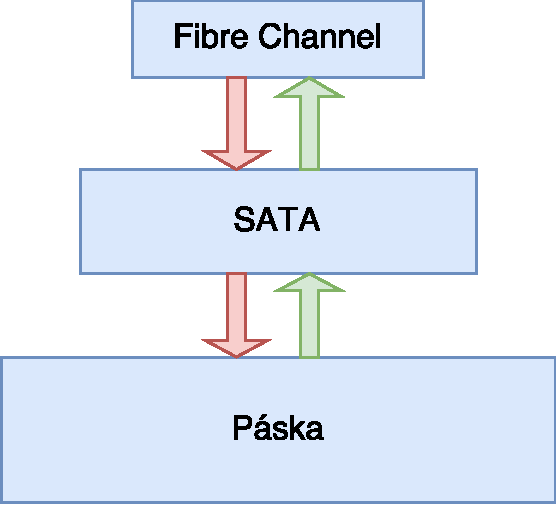
\includegraphics[width=50mm]{img/hie_zcu.pdf}
\caption{Hierarchické archivační úložiště CESNET HSM Plzeň}
\label{fig:hie_zcu}
\end{figure}

Jedním příkladem použití může být archivační úložiště CESNET HSM Plzeň na ZČU, jehož jednotlivé vrstvy jsou vidět na obrázku \ref{fig:hie_zcu}. Úložiště využívá 3 typy úložišť a to fibre channel, SATA a páska \cite{cesnetstor}.

\subsection{Zástupci}

V této podkapitole jsou uvedeni dva zástupci pro hierarchickou správu úložiště.

\subsubsection*{ZFS}

ZFS \cite{zfspaper} je jak souborovým systémem tak správcem logických disků\footnote{Možnost spojit více fyzických úložišť či diskových oddílů do logického celku}. Díky této kombinaci má kompletní přehled nejen o souborovém systému ale i o fyzických zařízeních, kterými je tvořen. Tato znalost umožňuje ZFS migrovat data na rychlejší úložiště podle potřeby. Migrace souborů probíhá automaticky a rozhoduje na základě četnosti přístupů k datům. Další z předností ZFS je možnost vytvářet snapshoty zachycující aktuální verzi souboru, ke kterým se následně můžeme vrátit bez ovlivnění chodu zbytku systému. 

\subsubsection*{HPSS}

HPSS \cite{hpssonline} je implementací hierarchického úložiště od firmy IBM. HPSS automaticky spravuje životní cyklus souborů a nepoužívaná data automaticky odsouvá na nejnižší vrstvy. Úložiště je navrženo pro clusterové využití, lze ho tedy jednoduše škálovat přidáním dalších uzlů. Pro práci s úložištěm lze využít speciální API nebo VFS.

\subsection{Shrnutí}

Hierarchický model uložení dat může zvýšit propustnost systému využitím rychlejší vrstvy úložiště, na které jsou umístěna často používaná data se zachováním velké kapacity úložiště použitím pomalejších, vysokokapacitních úložišť. Hierarchický model uložení dat ovšem postrádá některé výhody distribuovaného souborového systému, a to především replikaci dat. 

\section{Distribuovaný souborový systém s hierarchickým modelem uložení dat}

V sekci \ref{dfs} byly popsány distribuované souborové systémy a jejich výhody a nevýhody. Jednou z uvedených nevýhod je snížená propustnost dat. Snížení propustnosti může být způsobeno vyšší režií distribuovaného souborového systému, ale také současným přístupem několika klientů. 

Propustnost a latence souborového systému jsou kritické pro účely jako je streamování videí nebo shromažďování velkého množství naměřených dat, u kterých jsou přenášená obrovská množství dat často s vysokými časovými nároky na přenos. Při použití pomalejších mechanických disků (HDD) v systému s velkým počtem požadavků může docházet ke snížení propustnosti dat a zvýšení latence. Dražší úložiště založená na flash paměti (např. SSD) nebo úložiště na bázi paměti RAM dosahují značně vyšších propustností (přenosových rychlostí) a nižších latencí \cite{sniassdhdd}, ovšem za mnohem vyšší cenu GB (viz \ref{localstorage}). Při velkém množství dat proto ve většině případů není možné využít pouze tyto výkonnější úložiště, zejména kvůli vysokým finančním nárokům. 

Jedním z možných způsobů, jak zvýšit propustnost u distribuovaného souborového systému a zároveň zachovat realistické pořizovací náklady na HW, je kombinace spolu s hierarchickým modelem uložení dat. Tento systém by si zachoval výhodné vlastnosti distribuovaných systémů a zároveň by nabídl vysokou propustnost díky rychlým vrstvám úložišť. Cenou za zvýšení propustnosti přenosu dat je vyšší složitost systému a režie spojená s migrací souborů.

Distribuovaný souborový systém s hierarchickým modelem dat je předmětem výzkumu na katedře KIV, vedený p. Ing. Pešičkou. Prováděný výzkum je podnětem pro vznik simulátoru, na kterém bude možné odzkoušet vlastnosti systému a zároveň poskytne referenční model pro měření, který bude porovnán s několika dalšími modely distribuovaného souborového systému.

\subsection{Princip fungování}
Hierarchický model uložení dat může být použit bez zásadního ovlivnění principu fungování distribuovaného souborového systému. Hierarchické úložiště lze použít transparentně nebo jako součást distribuovaného souborového systému. 

V případě transparentního použití si hierarchické úložiště interně řeší migrování souborů a distribuovanému souborovému systému se jeví jako klasické úložiště. Tímto řešením bychom mohli dosáhnout zvýšení propustnosti při zachování nezávislosti mezi hierarchickým úložištěm a distribuovaným souborovým systémem.

Při použití hierarchického modelu uložení dat jako součásti distribuovaného souborového systému je výhodou možnost dělat rozhodnutí na základě stavu hierarchického úložiště. Systém bude moct během plánování migrace zohledňovat klientské požadavky a pokusit se podle nich optimalizovat rozmístění souborů na dostupné vrstvy. Jelikož má informace o probíhajících migracích souborů, může se během výběru cesty pro přenos dat pokusit vyhnout úložištím, která jsou aktuálně zpomalena migrací, volbou alternativní cesty. Na základě uvedených přínosů bylo vybráno zapojení hierarchického modelu dat jako součásti distribuovaného souborového systému.

\subsection{Vrstvy úložišť}
Při použití hierarchického modelu uložení dat budou úložiště každého serveru rozdělena podle výkonnostních parametrů (přenosové rychlosti) na několik vrstev, aby bylo možné využít rychlejších úložišť pro data, ke kterým je často přistupováno. K využití výhod hierarchického úložiště musí mít server alespoň 2 vrstvy úložišť, ze kterých budou data přístupná. Pokud má server pouze 1 vrstvu, bude fungovat jako klasický server bez hierarchického úložiště. Jelikož je počet vrstev individuální pro každý server, systém bude možné provozovat i v heterogenním prostředí.

\subsection{Migrace souborů}
Výkonnostní výhody hierarchického modelu uložení dat plynou z možnosti migrovat soubory mezi jednotlivými vrstvami úložišť. Migrace probíhá na základě použité migrační strategie (popsány v kapitole \ref{strategiemigrace}). Jako migrační strategie byla zvolena cachovací strategie, konkrétně poté algoritmus LFU, který nahrazuje data s nejmenším počtem přístupů. Zvolení konkrétní strategie závisí na předpokládaném použití systému a chování uživatelů. Pro naše potřeby předpokládáme, že uživatelé přistupují k rozsáhlému počtu různých dat, ale zároveň existuje množina dat, ke které přistupují častěji než k ostatním (oblíbená data).

Pro potřeby zvolené migrační strategie je nutné u každého souboru zaznamenávat počet přístupů. Při každém přístupu k souboru se zvýší čítač, na základě kterého bude vyhodnoceno, zda má být soubor odmigrován na vyšší vrstvu úložiště. Vyhodnocení, zda provést migraci souboru, může probíhat např. při každém přístupu k souboru nebo periodicky ve zvoleném intervalu. V případě použití úložných zařízení s rozdílnými rychlostmi čtení a zápisu lze navíc rozlišovat přístup typu čtení a přístup typu zápis.

Během migrace je soubor kopírován ze zdrojového úložiště na cílové. Je-li vyžádán soubor ze serveru, na kterém aktuálně probíhá migrace, bude soubor čten ze zdrojového úložiště, dokud se celý neodmigruje na cílové úložiště. Po dokončení migrace je soubor ze zdrojového úložiště odstraněn. Alternativou je ponechat soubor na zdrojovém úložišti a využít tak vyšší vrstvu pouze jako cache paměť. Tento přístup ovšem značně zvyšuje režii systému kvůli nutnosti zajisit konzistenci souboru mezi více vrstvami a snižuje celkové použitelné místo v systému.

Při zaplnění vyšší vrstvy úložiště musí být migrační strategie schopna určit množinu souborů, která bude muset být odmigrována na nižší úložiště, za účelem uvolnění místa. Jiným řešením při nedostatku místa může být migrace souboru na rychlou vrstvu úložiště jiného serveru. Toto řešení ovšem zvyšuje komplexitu systému a přináší dodatečnou režii při přenosu souborů mezi servery.


\chapter{Existující simulátory} \label{existujicisimulatory}

Jak je zřejmé z kapitoly \ref{ulozenidat}, existujících způsobů uložení je mnoho. Při návrhu a nasazení nového systému je tak komplikované odhadnout skutečné chování systému při očekávané zátěži. Stejně tak při vývoji nových funkcionalit dokážou simulátory dopředu napovědět, zda se implementace vyplatí či nikoliv. Z těchto důvodu existují simulátory, které se snaží věrohodně simulovat chování systému.

Mezi zmíněnými simulátory jsou i simulátory, které nejsou specializovány na simulaci úložišť, ovšem i přes to souvisí s touto prací.

\section{DiskSim} 

\textit{DiskSim} \cite{disksimdoc} je efektivní, přesný a vysoce konfigurovatelný simulátor úložných zařízení. Umožňuje simulaci disku, řadičů, sběrnic, ovladačů, plánovačů a dalších. Tento simulátor se specializuje na přesné simulování disků a jejich spolupráci s operačním systémem. Umožňuje konfiguraci plánování požadavků, cachování, organizaci dat na několika úrovních, jakými jsou například operační systém, řadič a samotný disk.

Pro běh simulace lze použít existující logy I/O požadavků nebo simulátorem vygenerované syntetické požadavky. DiskSim je vhodné použít pro ověření výkonnosti úložného systému, vlivu výkonnosti úložiště na celkový výkon systému a simulaci nových architektur úložného subsystému. 

Simulátor je zaměřen především na hardwarovou část úložiště. Simulátor ovšem nenabídne možnost simulace komplexnějších systémů pro uložení dat jako jsou například hierarchické či distribuované souborové systémy.

\section{OGSSim}

\textit{OGSSim} \cite{ogssimpaper} je simulátor inspirovaný simulátorem \textit{DiskSim} a snaží se řešit některé nedostatky tohoto simulátoru. Hlavním rozdílem je možnost simulovat komplexnější systémy s větším počtem úložišť a možnost kombinovat více technologií úložišť (např. HDD a SSD).

Konfigurace disků je možná v následujících formátech: JBOD, RAID1, RAID-01 a RAID (n+p), kde $n$ představuje počet disků s daty a $p$ počet disků s paritou. Dále umožní výběr strategie pro umísťování parity na disky v raidu. Jednotlivé disky nebo vytvořené svazky lze přiřadit do vrstev a tak simulovat hierarchický souborový systém. 

Simulátor se skládá ze 7 hlavních modulů:

\begin{itemize}

\item \textbf{Workload} Zpracovává požadavky ze vstupního souboru.

\item \textbf{Hardware Configuration} Načítá konfiguraci simulovaného systému z XML souboru.

\item \textbf{Simulation Configuration} Načítá konfiguraci simulátoru z XML souboru.

\item \textbf{Pre-processing} Předzpracování požadavků a spuštění simulace.

\item \textbf{Volume Driver} Modul řídící úložiště a jejich konfigurace.

\item \textbf{Device Driver} Simulace ovladače zařízení, implementuje hardwarově specifické vlastnosti.

\item \textbf{Execution} Vykonává požadavky směřované na jednotlivá úložiště.

\end{itemize}

Pro spuštění simulace jsou potřeba minimálně 3 vstupní soubory. Tento přístup umožní uživateli detailní popis simulovaného systému ovšem vytváření a orientace v konfiguračních souborech může být poměrně náročná. Hlavními výsledky jsou výkonnostní ukazatele, ale nabídne například i ukazatele spolehlivosti systému.

Simulátor je určený na simulaci rozsáhlých úložišť s detailní konfigurací hardwaru a použitých technologií spolu se simulací hierarchického úložiště. Součástí simulátoru není grafické prostředí a tak vyžaduje konfiguraci pomocí vstupních souborů. Stejně tak výsledky jsou prezentovány v textovém formátu. Simulátor ovšem neumožňuje simulaci distribuovaných souborových systémů.

\section{StorageSim}

\textit{StorageSim} \cite{storagesimpaper} je simulátor zaměřený na hierarchická úložiště. Umožňuje měření propustnosti  hierarchického modelu úložiště vs. klasické úložiště a ideální poměr velikostí rychlejší a pomalejší vrstvy pro výkon úložiště.

Simulátor má ve výchozím stavu 3 strategie migrace a to hashovací, cachovací a f4. Další strategie je možné doplnit díky modulárnímu návrhu. Simulace tedy umožňuje otestování navrhované strategie migrace před nasazením do reálného systému.

Simulované požadavky jsou čteny ze vstupního souboru ve formátu dostupného od asociace \textit{Storage Networking Industry Association (SNIA)}. Simulátor byl autory testován při simulaci reálného provozu vyhledávače \href{https://yahoo.com}{Yahoo}, který představoval téměř 55 miliónů diskových operací během 1 hodiny. Při testování byl StorageSim schopný zpracovat zhruba 8000 operací za sekundu.

Simulátor je více abstraktní než např. \textit{DiskSim} nebo \textit{OGSSim} za účelem zvýšení rychlosti simulace. Při simulaci jsou zanedbány věci jako jsou např. režie spojená s vytvářením či mazáním souborů, cachovací paměť a plánovač požadavků. Simulaci distribuovaných souborových systémů ovšem simulátor neumožňuje.

\section{Google File System Simulator}

\textit{Google File System Simulator} \cite{gfssimulatorpaper} je simulátor zaměřen na distribuovaný souborový systém Google File System (GFS). Primárním cílem simulátoru je ověřit chování a výkon GFS při různorodých zátěžích a podmínkách. Součástí simulace je simulace replikace souborů, vyvažování zátěže a simulace výpadku disku.

Simulace je založena na diskrétních událostech, kde každý požadavek je reprezentován událostí. Události jsou vybírány z fronty a postupně zpracovávány. 

Simulátor umožňuje volbu propustnosti spojení klienta se systémem od 0 do 1000 Mbps. Spojení mezi servery má neomezenou propustnost, což může být limitující faktor při modelování reálného systému. Simulátor je omezen pouze na jeden distribuovaný souborový systém bez možnosti simulace hierarchického modelu uložení dat.

\section{GridSim}

\textit{GridSim} \cite{gridsimpaper} je simulátor zaměřený na paralelní a distribuované výpočty. Umožňuje modelovat síťové spojení mezi uzly, různé typy zdrojů, uživatele, aplikace a plánovače. 

Dále slouží k porovnávání plánovacích algoritmy při simulované zátěži nebo k analýze zatížení různých zdrojů (procesor, disk). Parametry zdrojů mohou být individuálně nastaveny pro každý zdroj, čímž lze simulovat i heterogenní systémy. Simulátor je využíván jako podklad mnoha akademických výzkumů, také díky jeho modulární architektuře, která umožňuje uživatelům rozšíření o dodatečnou funkcionalitu. Výstupní formát výsledků simulace je řízen programátorem pomocí dat, která jsou mu zpřístupněna veřejným rozhraním simulovaných objektů. Simulátor neumožňuje simulovat distribuované souborové systémy s hierarchickým modelem uložení dat.

\section{Packet Tracer}

\textit{Packet Tracer} \cite{packettracerpaper} je nástroj pro simulaci počítačové sítě určený pro výuku. Umožňuje ruční modelování sítí, detailní analýzu datového toku, vizualizaci toku a volbu protokolů na jednotlivých vrstvách TCP/IP modelu. Simulace může probíhat v reálném čase nebo zrychleně.

\begin{figure}[H]
\centering
	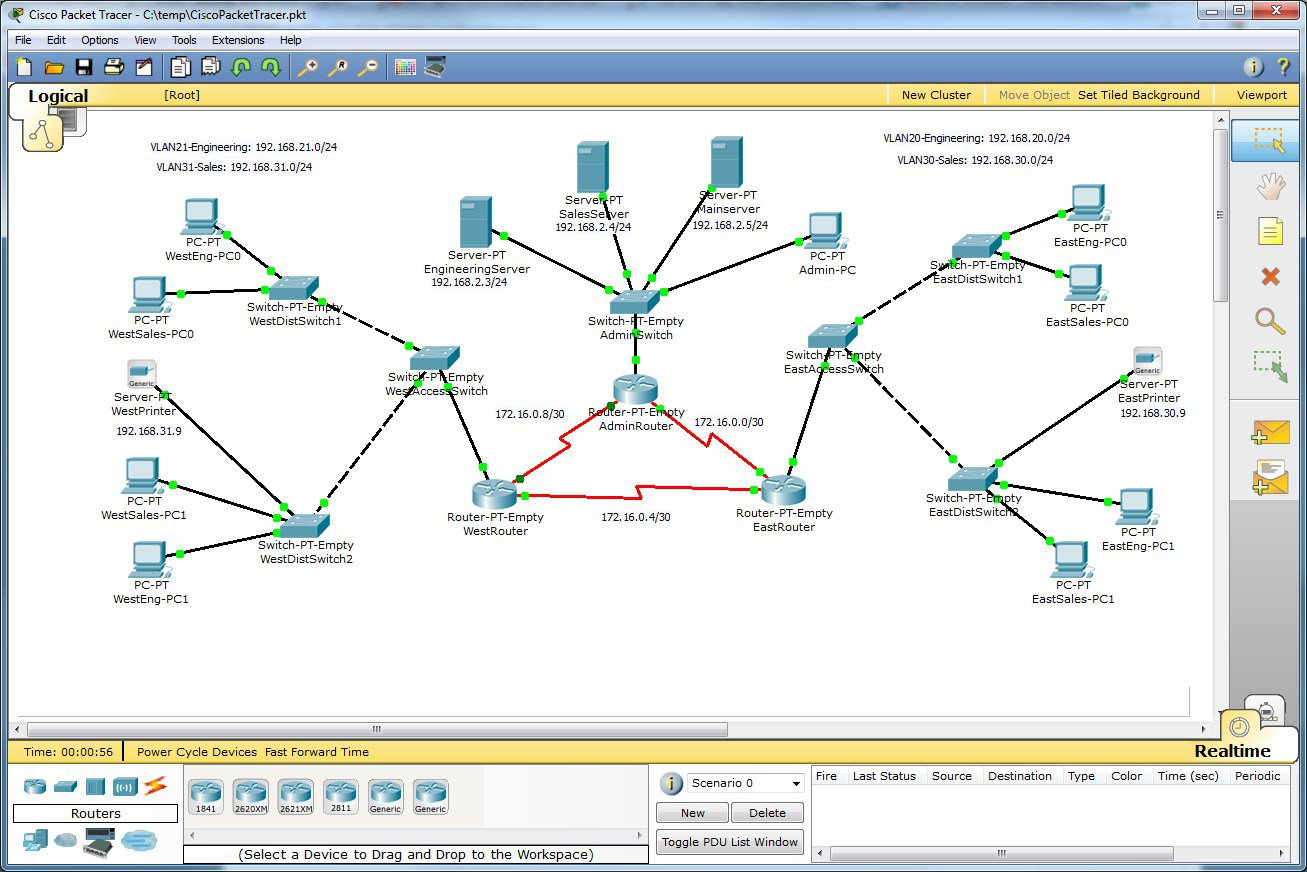
\includegraphics[width=\textwidth]{img/packet_tracer.jpg}
\caption{Ukázka modelování v Packet Tracer}
\label{fig:packet_tracer}
\end{figure}

Modelování simulovaného prostředí probíhá tažením myši prvků z knihovny (např. routery, switche) a následným propojením, viz obr. \ref{fig:packet_tracer}. Tento simulátor se nezaměřuje na simulaci úložiště a byl zkoumán a zmíněn hlavně kvůli inspiraci při návrhu vlastního simulátoru.

\section{Existujících simulátory a vlastní řešení}

Byly otestovány některé existující simulátory lokálních úložišť, hierarchických úložišť a simulátor konkrétního distribuovaného souborového systému. Simulace lokálních úložišť umožnila detailní hardwarové modelování a spolupráci hardwaru s operačním systémem. S rostoucí složitostí simulovaného systému se zvyšovala i abstrakce simulace hlavně z důvodů komplexnosti a rychlosti simulátoru. Pro distribuovaný souborový systém byl otestován simulátor simulující \textit{Google File System}, který je zaměřen pouze na tento souborový systém a tak jsou možnosti konfigurace poměrně omezené. 

\subsection{Vlastní řešení} \label{vlastnireseni}

Z otestovaných simulátorů se nejeví ani jeden jako vhodný kandidát na simulování obecných distribuovaných souborových systémů, proto bude v praktické části implementováno vlastní řešení. Simulátor by měl umožnit modelovat spojení mezi klientem a vnitřní propojení mezi servery, aby bylo možné simulovat reálný systém a jeho provozní vlastnosti. 

Vlastní řešení by mělo být schopné modelovat libovolnou strukturu distribuovaného souborového systému spolu s propojením serverů mezi sebou a mezi klientem a servery. Pro jednoduchost návrhu by mělo být součástí grafické rozhraní, které většině ze zmíněných simulátoru chybělo, pomocí něhož si bude moct uživatel systém nakonfigurovat a následně otestovat. 

Při návrhu vlastního řešení se můžeme inspirovat vhodnými vlastnostmi otestovaných simulátorů a to například detailními možnostmi konfigurace systému, možným porovnáním výsledků simulace s různými parametry simulovaného systému (např. strategie volby cesty, strategie migrace souborů), modulárním návrhem, který umožní jednoduché rozšíření simulátoru a grafickým rozhraním, které zajistí uživatelsky přívětivé modelování systému.

\subsubsection*{Shrnutí požadavků}

Vlastní simulátor by měl splňovat následující požadavky:

\begin{itemize}
\item umožnit modelovat spojení mezi servery a mezi servery a klientem,
\item umožnit modelovat libovolnou strukturu systému,
\item umožnit modelovat systém pomocí grafického rozhraní,
\item umožnit konfiguraci prvků systému a to serveru, klienta a spojení,
\item umožnit replikaci souborů mezi servery,
\item umožnit zobrazení výsledků simulace (průměrná rychlost, počet přenesených dat, graf průběhu rychlosti v závislosti na čase) pro jednotlivé testované metody,
\item umožnit simulovat hierarchický model uložení dat,
\item umožnit snadné rozšíření simulátoru modulárním návrhem.

\end{itemize}

\chapter{Návrh simulátoru}

Cílem simulace bude porovnat různé modely zapojení distribuovaných souborových systémů. Navržený simulátor se bude řídit požadavky uvedenými v kapitole \ref{vlastnireseni}.

\section{Struktura}

Simulátor se bude skládat z aplikační části a grafické části. Aplikační část bude zajišťovat běh simulace, sbírání výsledků a měření požadovaných veličin. Aplikační část by neměla být nijak závislá na grafické části. Díky oddělení těchto dvou částí bude v budoucnosti možné nahrazení grafického rozhraní bez nutnosti provádět změny v existujícím kódu simulátoru.

Grafická část umožní uživateli modelování distribuovaného systému z grafického rozhraní, vytváření plánu simulace, spuštění simulace a detailní zobrazení průběhu simulace a naměřených výsledků. Dále bude umožňovat exportování výsledků do formátu, aby s nimi bylo možné dále pracovat.

\section{Technologie}

Na základě požadavků na simulátor byly vybrány technologie pro implementaci. Aby se mohl simulátor dostat k většímu počtu uživatelů, neměl by být svázán s konkrétním operačním systémem. Cílem je tedy podpora alespoň všech hlavních operačních systémech a to \textit{MS Windows}\footnote{\url{https://www.microsoft.com/en-us/windows/}}, \textit{Linux}\footnote{\url{https://www.kernel.org/}} a \textit{Mac OS}\footnote{\url{https://www.apple.com/cz/macos/}}.

Stav simulátoru a modelovaný distribuovaný souborový systém by mělo být možné exportovat, aby se měření mohla opakovat. Modelování rozsáhlého systému může být časově velice náročné a tak by měl být formát uloženého stavu simulátoru strojově zpracovatelný, díky čemuž bude možné strojově generovat modely.

Jako programovací jazyk jsem zvolil jazyk \textit{Java}, konkrétně \textit{Java 8}\footnote{\url{http://www.oracle.com/technetwork/java/javase/overview/java8-2100321.html}} spolu s platformou \textit{JavaFX} \cite{javafxbook} pro vývoj grafického rozhraní. Java umožní běh na požadovaných operačních systémech a platforma \textit{JavaFX} zajistí jednotný vzhled napříč těmito systémy. Základní funkčnost simulátoru bude otestována pomocí Unit testů frameworkem \textit{JUnit} \cite{unittestpaper}.

Popis stavu simulátoru a modelovaného distribuovaného souborového systému bude řešen pomocí jazyka značkovacího \textit{XML}\footnote{\url{https://www.w3.org/XML/}}. Jazyk \textit{XML} je jednoduše vytvářen a zpracován standardními knihovnami Javy.

\section{Modelování systému}

Model systému bude reprezentován grafem. Uzly grafu budou dvojího typu a to buď klient nebo server. Hrany mezi uzly představují propojení pomocí počítačové sítě. Pro modelování distribuovaného souborového systému budou použity následující komponenty:

\begin{itemize}

\item \textbf{Klient} Představuje klienta, který komunikuje se servery distribuovaného souborového systému.

\item \textbf{Server} Představující jeden server distribuovaného souborového systému.

\item \textbf{Úložiště} Každý server může mít libovolný počet úložišť. Úložiště bude mít parametry rychlost (čtení i zápis) a velikost.

\item \textbf{Složka} Složka bude sloužit pro organizaci struktury dat v systému. Složku bude mít jméno a bude jí možné připojit na libovolné existující úložiště serveru.

\item \textbf{Soubor} Soubor má jméno a velikost. Musí mít rodiče typu složka. Jeden soubor může být umístěn (replikován) na více serverů.

\item \textbf{Linka} Linka představuje spojení mezi serverem a klientem, její parametry jsou rychlost a odezva.

\item \textbf{Charakteristika linky} Slouží k simulaci zatížení linky v čase. Bude určovat skutečnou propustnost.

\end{itemize}

\section{Modularita}

Simulátor by měl mít modulární strukturu, aby byla možná jednoduchá implementace dalších metod výběru cesty, strategií migrace souborů v hierarchickém modelu uložení dat a grafického klienta (např. specializovaný klient pro rozsáhlé systémy).

\section{Formát výstupu}

Výstup simulace by měl být ve strojově zpracovatelném formátu ale zároveň by mělo být uživateli umožněno přímo v prostředí simulátoru zobrazit výsledky pomocí grafu.

\section{Rozsah simulovaného systému}

Simulátor by měl být schopný simulovat jak miniaturní systémy tak systémy o velkém počtu serverů a velkém počtu požadavků na přenos dat. Během simulace by měl být uživatel informován o průběhu v grafickém prostředí a po dokončení o výsledcích. Jelikož bude simulátor dimenzován na velký počet serverů a požadavků, měla by vizualizace průběhu doběhnout v rozumném čase nebo uživateli nabídnout možnost ji přeskočit.

\chapter{Implementace aplikační části}

V následující části je popsána implementace a detaily aplikační části, tedy části programu, která řídí modelování systémů a běh simulace. Všechny cesty k balíkům, které jsou v této části odkazovány, jsou pouze relativní cesty k rodičovskému balíku \textit{cz.zcu.kiv.dfs\_simulator}.

\section{UML diagram}

Na následujících obrázcích \ref{fig:uml_simulace} a \ref{fig:uml_uloziste} jsou znázorněny pomocí UML diagramu nejdůležitější části aplikační části simulátoru, samotný simulátor respektive model serveru a úložiště.

\begin{figure}[H]
\centering
	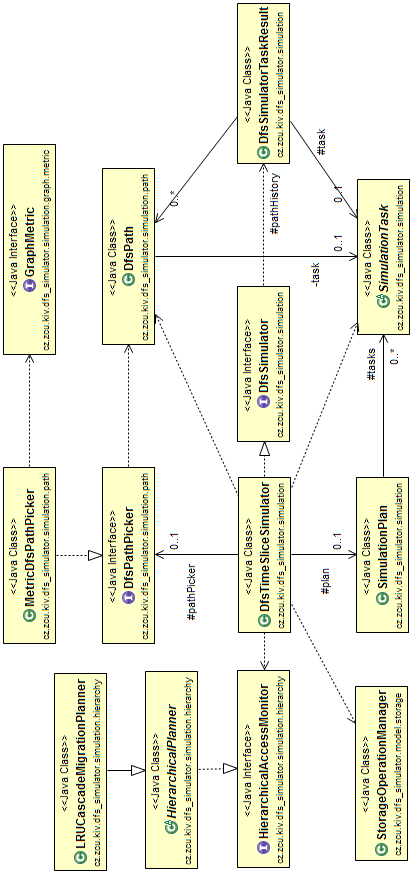
\includegraphics{img/uml_simulace.png}
\caption{UML diagram simulační části}
\label{fig:uml_simulace}
\end{figure}

\begin{figure}[H]
\centering
	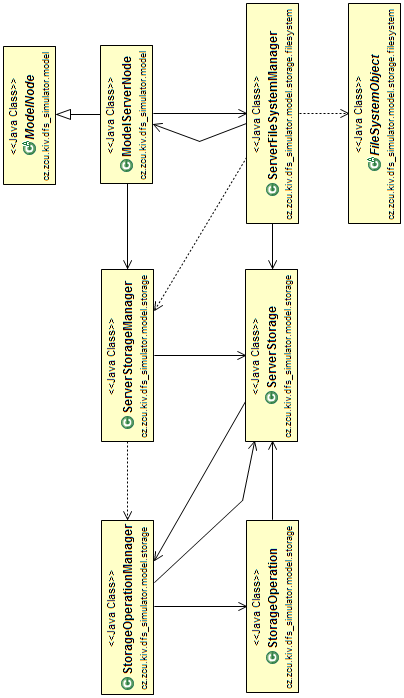
\includegraphics{img/uml_uloziste.png}
\caption{UML diagram serveru a úložiště}
\label{fig:uml_uloziste}
\end{figure}

\section{Model}

Modelovací část poskytuje prvky k modelování distribuovaného souborového systému. Modelovaný systém je interně reprezentován jako orientovaný graf (důvod popsán v \ref{propojeniuzlu}). Hrany grafu mají ohodnocení kombinované z propustnosti a latence spojení. Zdrojové soubory modelu jsou obsaženy v balíku \textit{model}.

\subsection{Jednotky rychlosti a velikosti}

Přenosová rychlost je reprezentována objekty třídy \textit{ByteSpeed}. Výchozí jednotkou je 1 byte/s, ale součástí třídy jsou metody pro získání hodnoty v násobcích kilobyte/s, megabyte/s a gigabyte/s. Velikost je obdobně reprezentována třídou \textit{ByteSize}. Výchozí jednotkou velikosti je 1 byte a součástí třídy jsou opět metody pro získání násobků kilobyte, megabyte a gigabyte. Násobky předpon jsou uvedeny v tabulce \ref{predpony_jednotky}.

\begin{table}[H]
\centering
\caption{Předpony jednotek}
\label{predpony_jednotky}
\begin{tabular}{|l|l|l|}
\hline
\textbf{Předpona} & \textbf{Násobek} & \textbf{$10^n$} \\ \hline
B                 & 1                & $10^0$       \\ \hline
kB                & 1000             & $10^3$          \\ \hline
mB                & 1 000 000        & $10^6$          \\ \hline
gB                & 1 000 000 000    & $10^9$          \\ \hline
\end{tabular}
\end{table}

\subsection{Uzly}

Uzly grafu dědí od rodičovské třídy \textit{ModelNode} a mohou být dvou typů a to klient nebo server. Uzly grafu, které mezi sebou mají hranu, představují sousedy a mohou spolu komunikovat. Uzly jsou registrovány do globálního registru \textit{ModelNodeRegistry}, aby byly viditelné ostatním částem simulátoru. Registrace uzlu probíhá pomocí unikátního identifikátoru typu \textit{StringProperty}.

\subsubsection*{Server}

Server je reprezentován třídou \textit{ModelServerNode} a v distribuovaném souborovém systému zastupuje datový server, který může mít neomezené množství různých úložišť a na nich uložena data. Každý server má vlastní kořenovou složku, která je kořenem adresářové struktury serveru, správce úložišť a správce adresářové struktury.

\subsubsection*{Klient}

Klient je uživatel, který může vytvářet požadavky na čtení nebo zápis souborů z některého ze serverů. Seznam požadavků klienta tvoří simulační plán a je uložen v objektu třídy \textit{SimulationPlan}. 

\subsection{Propojení uzlů} \label{propojeniuzlu}

Logika pro propojení uzlů je v samostatném balíku \textit{connection}. Jednotlivé uzly mohou být propojeny instancemi třídy \textit{ModelNodeConnection}. Propoj je orientován z výchozího do cílového uzlu, díky čemuž lze vytvářet mezi uzly nesymetrické propoje. Nesymetrické propoje mohou představovat například připojení typu ADSL, které mají často několikrát větší rychlost stahování než nahrávání. Dalšími vlastnostmi propoje je maximální propustnost dána instancí třídy  \textit{ByteSpeed}, latence v milisekundách a zátěžová charakteristika (viz \ref{zatezovacharakteristika}). Latence propoje udává za jak dlouhou dobu obdržíme odpověď od protějšku po vyslání požadavku (např. ICMP ping).

\subsection{Zátěžová charakteristika propojení uzlů} \label{zatezovacharakteristika}

Zátěžová charakteristika propoje slouží k simulaci zátěže v závislosti na běžícím čase simulace. Implementace charakteristiky musí implementovat rozhraní \textit{ConnectionCharacteristic} a jeho metody. V závislosti na konkrétní implementaci může být charakteristika jednorázová nebo periodická. Výchozí implementací je periodická lineární charakteristika definována pomocí několika diskrétních bodů.

\subsubsection*{Rozhraní ConnectionCharacteristic}

Rozhraní \textit{ConnectionCharacteristic} má následující metody:

\begin{verbatim}
double getAverageBandwidthModifier(long sTime, 	
      long intervalLength);
    
void setPeriodInterval(long time);
LongProperty periodIntervalProperty();
    
double getYLowerBound();
double getYUpperBound();
    
double getXLowerBound();
double getXUpperBound();
\end{verbatim}

\noindent Metoda \textit{getAverageBandwidthModifier} vrací průměrný modifikátor propustnosti v časovém intervalu $sTime, sTime + intervalLength$, \textit{setPeriodInterval} nastavuje délku časového intervalu charakteristiky (u periodických nastavuje délku periody). Metody \textit{getYLowerBound}, \textit{getYUpperBound} a \textit{getXLowerBound}, \textit{getXUpperBound} vrací rozmezí osy $X$ (čas), resp. $Y$ (modifikátor).

\subsubsection*{LineConnectionCharacteristic}

\textit{LineConnectionCharacteristic} je implementace zátěžové charakteristiky, konkrétně lineární periodická charakteristika, využívající několik diskrétních bodů propojených úsečkami (po částech lineární funkce). Na ose $x$ je průběh času a na ose $y$ je modifikátor propustnosti v intervalu $<0.01, 1>$.

\begin{figure}
\centering
	\fbox{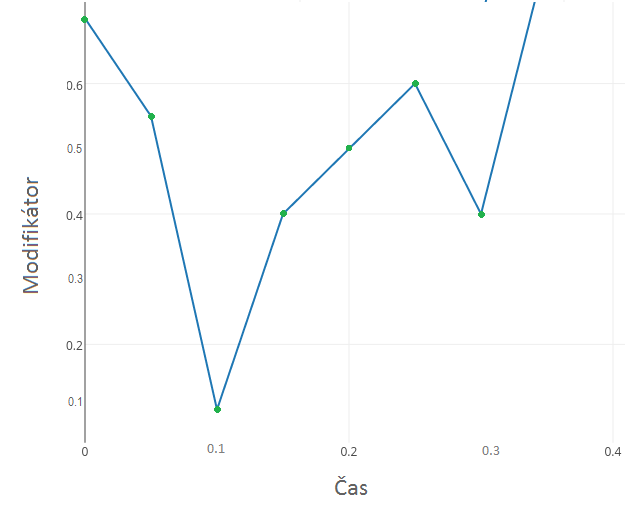
\includegraphics[width=100mm]{img/linearni_charakteristika.png}}
\caption{Lineární zátěžová charakteristika}
\label{fig:lin_charakteristika_propoje}
\end{figure}

Na obrázku \ref{fig:lin_charakteristika_propoje} je zobrazena část charakteristiky. Pokud bychom tedy měli linku s maximální propustností 10 mB/s a zajímala by nás skutečná propustnost v čase 0.2, vynásobíme maximální propustnost hodnotou 0.5 a získáme 5 mB/s.

Pokud bychom chtěli zjistit propustnost v čase, ve kterém přímo neleží některý z definovaných bodů, je využito následujících rovnic: 

\begin{equation}\label{eq:mod_lin}
mod = A_y(1 - t) + B_yt
\end{equation}

\begin{equation}
t = (B_x - A_x) / (d_x - A_x)
\end{equation}

\noindent kde $d_x$ je hledaný čas, $A$ a $B$ jsou body ležící na časovém intervalu, do kterého spadá námi hledaný čas a $t$ je normalizovaná vzdálenost hledaného času od výchozího bodu $A$.

Pokud bychom hledali modifikátor v čase $d_x = 0.225$ (obr. \ref{fig:lin_charakteristika_propoje}) musíme nalézt mezilehlé body, které jsou v našem případě $A = (0.2,0.5) $ a $B = (0.25, 0.6)$. 

\noindent Výpočet vzdálenosti $t$:

\begin{equation}
t = (0.25 - 0.2) / 0.25 = 0.5
\end{equation}

\noindent Výpočet modifikátoru v čase $d_x$:

\begin{equation}
mod = 0.5(1 - 0.5) + 0.6 * 0.5 = 0.55
\end{equation}

\subsection{Adresářová struktura}

Pomocí adresářové struktury jsou na serverech uspořádána data. Adresářová struktura je stromem, jehož kořenem je kořenová složka $/$ příslušného serveru, tedy obdobně jako na UNIXových systémech. Implementace adresářové struktury a věcí s ní společných je obsažena v balíku \textit{storage.filesystem}.

\subsection{Správce adresářové struktury}

Adresářová složka je spravována objektem třídy \textit{ServerFileSystemManager}, který spravuje všechny datové objekty (soubory či složky) uložené na serveru. Interně je mapování datových objektů na úložiště realizováno pomocí mapy \textit{HashMap}, jejímž klíčem je instance datového objektu a hodnotou úložiště. Součástí jsou zároveň pomocné metody na přidávání nových potomků do adresářové struktury serveru, které hlídají dostupné místo na patřičném úložišti a v případě nedostatku je vyvolána výjimka typu \textit{NotEnoughSpaceLeftException}.

\subsubsection*{Cesta}
Cesta souboru nebo složky je tvořena rekurzivně přes rodiče až ke kořeni stromu a jednotlivé vrcholy jsou odděleny pomocí oddělovače $/$. Pro soubor $f1$ ve složce $d1$ by výsledná cesta byla $/d1/f1$ a pro složku $s1$ ve složce $d1$ poté $/d1/s1/$. Jak je vidět, tak cesty složek končí oddělovačem $/$.

\subsubsection*{Implementace datových objektů}
Datové objekty jsou reprezentovány abstraktní třídou \textit{FileSystemObject}, konkrétně potom \textit{FsFile} a \textit{FsDirectory} pro soubor respektive složku. Každý objekt má jméno, které je unikátní na dané úrovni ve stromové struktuře a rodiče typu složka. Soubory mají navíc ještě velikost a čítač přístupů. Jediný objekt, který nemá rodiče, je kořenová složka.

\subsubsection*{Vyhledávání}
Vyhledávání souborů v adresářové struktuře serveru lze provést metodou objektu třídy FsDirectory

\begin{verbatim}
FileSystemObject getChildObject(String path)
\end{verbatim}

\noindent která prohledává potomky dané složky. Hledáme-li od kořenové složky, cesta musí začínat $/$. Na nižších úrovních předáváme pouze relativní cestu bez počátečního $/$, tedy například pro soubor s absolutní cestou $/d1/s1/f1$ bychom při hledání od kořene použili celou absolutní cestu a při hledání ze složky $d1$ relativní cestu $s1/f1$.

\subsubsection*{Registr datových objektů}
Pro jednoduchost jsou všechny datové objekty registrovány do globálního registru \textit{FsGlobalObjectRegistry}, který mapuje cesty datového objektu na objekty instance \textit{ObjectRegistryEntry}. V objektu třídy \textit{ObjectRegistryEntry} jsou seznamy serverů a instancí třídy \textit{FileSystemObject} pro každou cestu.

\subsection{Replikace}

Replikace souborů je implementována v balíku \textit{storage.replication}. Pokud sdílí více souborů absolutní cestu na několika serverech, jsou jejich instance považovány za repliky jednoho souboru. Správu replik zajišťuje třída \textit{FsGlobalReplicationManager}, která poskytuje metody pro získání všech instancí replik jednoho souboru, přejmenování replik, mazání a měnění velikosti replik.

Repliky se řídí optimální strategií - všechny repliky jsou RW, lze tedy zapisovat do libovolné instance. Po přepsání vybrané instance repliky dochází k propagaci změn ze serveru s vybranou replikou na zbylé instance (synchronizace). Při synchronizaci replik jsou vytvořeny diskové operace na čtení (zdrojový server) a zápis (cílové servery).

\subsection{Úložiště}

Úložiště a s ním spojené operace jsou implementovány v balíku \textit{storage}. Samotné úložiště je implementováno třídou \textit{ServerStorage}, která má danou velikost, maximální přenosovou rychlost sdílenou pro čtení a zápis a vlastní instanci správce I/O operací (viz \ref{ioop}).

Úložiště jako takové neví nic o datech, která jsou na něm uložena. Informace o datech jsou součástí adresářové struktury a ta je spravována pro každý server individuálně pomocí objektu \textit{ServerFileSystemManager}.

\subsubsection*{Správce úložišť}

Správce úložišť, implementován třídou \textit{ServerStorageManager}, uchovává seznam všech úložišť daného serveru, ke kterému správce patří. Pomocí správce lze provádět hromadné operace nad úložišti jako jsou např. metody pro komunikaci se správcem I/O operací jednotlivých disků. 

\subsection{I/O operace} \label{ioop}

I/O operace \textit{StorageOperation} jsou operace čtení a zápisu na konkrétním úložišti. Operace jsou interně rozlišeny pomocí výčtového typu \textit{StorageOperationType} a aktuálně mohou být 4 druhy operací: READ, WRITE, CLIENT\_READ a CLIENT\_WRITE. Operace s předponou \textit{CLIENT} jsou operace, které nejsou automaticky spravovány (jak bude popsáno dále v „Správce operací“). Ke každé operaci je přiřazen seznam přenášených souborů, maximální rychlost operace, přidružená operace na jiném disku, seznam navazujících operací a callback.

\subsubsection*{Správce operací}

I/O operace jsou spravovány třídou \textit{StorageOperationManager}. Hlavním účelem správce operací je výpočet dostupné rychlosti a počtu přenesených dat u každé operace. Správce je unikátní pro každé úložiště a spravuje dva seznamy operací - běžící operace a čekající operace. Čekací operace jsou operace, které čekají na dokončení některé rodičovské operace, která může aktuálně čekat či běžet.

Řízení operací je rozlišeno spravovanými a nespravovanými operacemi. Oba typy operací jsou v příslušných frontách, ovšem u nespravovaných operací není správcem řízen jejich průběh (přenesená data). Nespravované operace jsou využívány v situacích, kdy se operace nemusí dokončit celá, tedy např. při přenosu ke klientovi a zapnutém dynamickém routováním.

\subsubsection*{Výpočet rychlosti operací}

Výpočet rychlosti operací je explicitně spouštěn uvnitř třídy \textit{StorageOperationManager} pro aktuálně běžící operace (i nespravovaného typu), konkrétně metodou

\begin{verbatim}
void updateAvailableThroughput(long sTime).
\end{verbatim}
Rychlost je operacím přidělována spravedlivě - maximální rychlost disku je dělena počtem všech operací. V případě, že má operace nastavenou omezující maximální rychlost, je nevyužitý díl rychlosti rozdělen mezi zbylé operace. 

\subsubsection*{Výpočet přenesených dat}

Výpočet přenesených dat probíhá explicitně uvnitř třídy \textit{StorageOperationManager} pro aktuálně běžící spravované operace, konkrétně metodou

\begin{verbatim}
void updateTransferedSize(long timeInterval, long sTime),
\end{verbatim}

\noindent která aktualizuje pro každou běžící operaci počet přenesených dat v intervalu daném proměnnou \textit{timeInterval}. Jako přenosová rychlost je použita vypočtená rychlost v metodě \textit{updateAvailableThroughput}. Po  dokončení je operace odebrána ze seznamu běžících operací a je vyvolán její callback, pokud má nějaký nastaven.

\subsubsection*{Přidružené operace}

Přidružené operace slouží k propojení dvou diskových operací a jsou využívány v případě, kdy se data přesouvají mezi úložišti, tedy např. při hierarchické migraci dat. Jelikož se může stát, že jedna z operací má větší dostupnou rychlost než druhá, musí být operace propojeny a jejich společná maximální rychlost je minimem z maximálních rychlostí samotných operací. 

Diskové operace hierarchické migrace lze vytvořit metodou \textit{addMigrationOperation} z instance správce operací, která zajistí vytvoření příslušných operací a jejich přidružení.

\subsubsection*{Navazující operace}

Pomocí navazujících operací lze vytvářet řetězec operací, které musí být vykonány popořadě. Navazující operace jsou využívány např. u hierarchické migrace dat v případě, kdy je nejdříve třeba z vyšší vrstvy data odmigrovat na vrstvu nižší, aby se uvolnil dostatek místa. 

Každá disková operace může mít neomezený počet navazujících operací. Navazující operaci lze přidat k instanci \textit{StorageOperation} metodou

\begin{verbatim}
void addFollowingOperation(StorageOperation followingOperation).
\end{verbatim} 

\noindent Po dokončení rodičovské operace jsou navazující operace automaticky správcem operací zařazeny do běžících operací.

\subsubsection*{Callback}

Callback je funkce, která je předána do instance diskové operace a očekává se její zavolání při určité události. Ve skutečnosti je implementována přes abstraktní třídu \textit{StorageOperationCallback}, která má dvě metody

\begin{verbatim}
abstract void onOperationStarted(long sTime)
abstract void onOperationFinished(long sTime).
\end{verbatim}

\noindent Metoda \textit{onOperationStarted} je vyvolána správcem operací před převedením diskové operace do běžícího stavu a metoda \textit{onOperationFinished} je vyvolána po dokončení běhu operace. Obě metody mají jako parametr aktuální čas simulátoru.

Callback funkce umožňují automatické provedení kódu, který si přejeme vykonat až při specifikované události. Při vytváření operace nejsme schopni předem určit v který čas operace začne (navazující operace) a kdy doběhne (závisí na dostupné rychlosti). Callback funkce jsou využívány např. u hierarchické migrace, kde je vytvořeno několik navazujících operací, které vyžadují po dokončení provést aktualizaci mapování souboru na úložiště.

\section{Simulace}

Logika řídící simulaci je obsažena v balíku \textit{simulation}. Hlavní součástí simulace je simulátor implementující rozhraní \textit{DfsSimulator}. Spolu se simulací probíhá logování všech důležitých akcí, díky kterému lze detailněji prozkoumat výsledek simulace a vzorkování rychlosti, které umožní náhled na průběh přenosové rychlosti v čase.

\subsection{Diskrétní událostní simulátor}

Implementovaným diskrétním událostním simulátorem je \textit{DfsTimeSliceSimulator}. Simulace probíhá jako sled událostí, kde události představují požadavky klienta na čtení nebo zápis souboru. Parametry simulátoru jsou simulační plán \textit{SimulationPlan}, instance \textit{DfsPathBuilder} zprostředkovávající výběr cesty od klienta k serveru a výčtový typ \textit{SimulationType} detailněji specifikující typ simulace (\ref{typysimulace}).

Vstupní simulační plán obsahuje klientské požadavky, které při simulaci představují události a jsou vykonávány postupně jedna po druhé. Zpracovávané požadavky jsou simulátorem krokovány, jelikož nelze dopředu jednoduše určit, jaký bude mít požadavek průběh kvůli proměnlivé propustnosti spojení a měnící se přenosové rychlosti disků v závislosti na existujících diskových operacích. 

Krok simulátoru je určen konstantou \textit{TIME\_RESOLUTION\_MS}, která má ve výchozím nastavení hodnotu 500 ms. Výběr velikosti je kompromisem mezi rychlostí běhu simulace a přesností simulace. Kratší simulační krok způsobí větší počet výpočtů pro každou událost a větší paměťové nároky pro uchování všech vzorků rychlosti. Delší simulační krok může mít negativní vliv na přesnost simulátoru, a to na navzorkované hodnoty rychlosti a na přesnost průběhu diskových operací, které jsou aktualizovány při každém kroku.

\subsection{Stahování a nahrávání souborů}

Klientské požadavky jsou reprezentovány abstraktní třídou \textit{SimulationTask}, konkrétně \textit{GetSimulationTask} a \textit{PutSimulationTask} pro stahování resp. nahrávání. Parametrem každého požadavku je objekt \textit{FsFile}, který se stahuje nebo nahrává.

V případě stahování se cílové úložiště určuje podle toho, na kterém úložišti je soubor uložen. Při nahrávání souboru je cílové úložiště zděděné od rodičovské složky, do které je soubor nahráván.

\subsection{Výsledky simulovaných požadavků} \label{vysledkypozadavku}

Výsledkem běhu simulátoru je seznam \textit{DfsSimulatorTaskResult}, kde každá položka seznamu je výsledek jednoho simulovaného požadavku. Výsledek obsahuje referenci na požadavek \textit{SimulationTask}, výčtový typ \textit{DfsSimulatorTaskResultState} určující stav výsledku, celkový čas pro vykonání požadavku, historii cest, přes které byl požadavek (soubor) přenášen a vzorky rychlosti. 

\noindent Simulace požadavku může skončit některým z následujících stavů:

\begin{itemize}
\item \textbf{SUCCESS} úspěšné dokončení požadavku
\item \textbf{NO\_NEIGHBOURS\_AVAILABLE} klient nemá žádné spojení se servery
\item \textbf{NO\_PATH\_AVAILABLE} k serveru nebo serverům, na kterých se nachází požadovaný soubor, neexistuje cesta
\item \textbf{NOT\_ENOUGH\_SPACE\_ON\_DEVICE} na nahrání souboru není na cílovém úložišti dostatek volného místa
\item \textbf{OBJECT\_NOT\_FOUND} pokud v cílové cestě nebylo nic nalezeno.
\end{itemize}

\subsection{Metoda simulace} \label{typysimulace}

Metoda simulace určuje, jaká metrika bude použita pro nalezení cesty, zda je zapnuto dynamické routování, interval přepočtu cest u dynamického routování a zda je během simulace povoleno hierarchické migrování souborů. Metodu simulace lze specifikovat výčtovým typem \textit{SimulationType}, který je použit jako vstupní parametr do simulátoru.

\subsection{Výběr cesty}

Během každého simulovaného požadavku se simulátor snaží nalézt cestu od klienta k jednomu z datových serverů, na kterém se nachází cílová cesta. K nalezení cesty u simulátoru \textit{DfsTimeSliceSimulator} je využíván parametr konstruktoru typu \textit{DfsPathPicker}. Při nalezení cesty je vždy na začátku započtena celková latence cesty k výslednému času simulace požadavku.

\subsubsection*{DfsPathPicker}

\textit{DfsPathPicker} popisuje rozhraní, které musí implementovat třída umožňující výběr cesty. Samotný DfsPathPicker se nestará o nalézání všech možných cest, pouze o výběr nejlepší cesty ze všech dostupných. Rozhraní nabízí následující metody:

\begin{verbatim}
DfsPath selectPath(SimulationTask task, long sTime, 
     DfsPath previousPath, SimulationType simType)

long getObjectRegistryQueryTime().
\end{verbatim}

\noindent Metoda \textit{selectPath} slouží k výběru nejlepší cesty a jejími parametry jsou simulovaný požadavek, již používaná cesta (je-li nastavena, metoda musí vrátit cestu vedoucí do stejného cílového serveru) a typ simulace. Pokud \textit{selectPath} vrátí hodnotu \textit{null}, znamená to, že nebyla nalezena žádná cesta a simulátor připočte k času simulace hodnotu vrácenou metodou \textit{getObjectRegistryQueryTime}, která vrací čas potřebný k dotázání na existenci souboru či složky jednoho ze serverů.

\subsubsection*{MetricDfsPathPicker}

Výchozí implementací \textit{DfsPathPicker} pro výběr cesty je \textit{MetricDfsPathPicker}, který využívá objektu implementující rozhraní \textit{GraphSearcher} pro vyhledávání cest. Při výběru cesty nejdříve zjistí všechny cílové servery, na kterých se nalézá požadovaná cesta a poté pro každý server nechá \textit{GraphSearcher} nalézt optimální cestu. Ze všech cest poté vybírá tu nejoptimálnější porovnáním jejich ohodnocení.

\subsubsection*{Dynamické routování}

Má-li typ běžící simulace zapnuté dynamické routování, simulátor musí po určité době provést opětovně výběr nové cesty. V případě nahrávání souborů musí mít nová cesta stejný cílový server (tzn. nahrávání se musí vždy dokončit na tom serveru, na kterém začalo). Interval přepočtu cest lze získat z \textit{SimulationType} metodou

\begin{verbatim}
int getDynamicPathingRecalcInterval(),
\end{verbatim}

\noindent která vrací hodnotu v milisekundách. Simulátor tedy v každém kroku simulace požadavku kontroluje, zda je třeba provést přepočet cest. Pokud je vybrána nová cesta, je k výslednému času opět připočtena latence cesty a nová cesta je uložena do seznamu, který uchovává historii cest daného požadavku.

\subsection{Vyhledávání v grafu}

Vyhledání cesty od klienta k cílovému serveru představuje problém nalezení optimální cesty v orientovaném ohodnoceném grafu pomocí zvolené metriky. Prohledávání v grafu zajišťuje objekt implementující rozhraní \textit{GraphSearcher}, které má následující metody:

\begin{verbatim}
Long findPath(ModelNode origin, ModelServerNode target, 
     SimulationTask task, long sTime, 
     List<ModelNodeConnection> path, SimulationType simType)
     
GraphMetric getMetric().
\end{verbatim}

\noindent Metoda \textit{findPath} slouží k nalezení cesty z výchozího uzlu \textit{origin} do cílového serverového uzlu \textit{target} a metoda \textit{getMetric} vrací metriku, která byla použita při hledání cesty.

\subsubsection*{DijkstraGraphSearcher}

Třída \textit{DijkstraGraphSearcher} je implementací \textit{GraphSearcher} sloužící k nalezení optimální cesty pomocí algoritmu vycházejícího z Dijkstrova algoritmu \cite[Sekce~24.3]{dijkstrabook}. 

Dijkstrův algoritmus byl zvolen na základě potřeby nalézt optimální cestu z jediného výchozího uzlu v grafu s kladně ohodnocenými hranami. Složitost Dijkstrova algoritmu je $O(|V^2|)$, kde $|V|$ je celkový počet uzlů. Alternativami mohou být například algoritmy Bellman-Fordův algoritmus ($O(|V||E|)$, kde $|E|$ je celkový počet hran) \cite{bellmanfordpaper} nebo Floyd-Warshallův algoritmus \cite{floydwarshall} ($O(|V^3|)$).

Hrany mezi uzly jsou hodnoceny metrikou \textit{GraphMetric}, která zároveň poskytuje komparátor pro výběr nejlepší hrany. Lze tedy hledat cesty podle více kritérií a nejsme omezeni pouze výběrem nejkratší, jak je tomu u základní verze algoritmu.

\subsection{Metrika grafu}

Metrika je využívána při prohledávání grafu k nalezení optimální cesty a je reprezentována objektem implementující rozhraní \textit{GraphMetric}.

\subsubsection*{Dostupné metriky}

V základní verzi simulátoru je implementováno následujících 6 metrik pro nalezení cesty:

\begin{itemize}

\item \textbf{DistanceMetric} Metrika sloužící k nalezení nejkratší cesty.

\item \textbf{LinkBwMetric} Metrika sloužící k nalezení cesty s největší propustností (nejširší cesta).

\item \textbf{LinkBwLatencyMetric} Metrika kombinující nalezení cesty s největší propustností a zároveň nejmenší latencí.

\item \textbf{PathThroughputMetric} Metrika kombinující nalezení cesty s největší propustností a zároveň s nejrychlejším diskem.

\item \textbf{PathThroughputLatencyMetric} Podobně jako \textit{PathThroughputMetric}, ovšem minimalizuje zároveň latenci.

\item \textbf{HierarchicalThroughputMetric} Podobně jako \textit{PathThroughputLatencyMetric}, ale vybírá cestu s ohledem na maximální možnou propustnost disku po provedení hierarchické migrace, tedy např. pokud je stahovaný soubor \textit{f1} na serverech \textit{S1} a \textit{S2}, kde na S1 má disk rychlost 100 MB/s a na S2 také 100 MB/s s tím, že na S2 existuje rychlejší disk 150 MB/s, který má volné místo, bude vybrána cesta k S2.

\end{itemize}

\subsubsection*{Popis rozhraní}

Rozhraní má následující metody:

\begin{itemize}

\item \textbf{getBestMetricValue} vrací nejlepší ohodnocení hrany
\item \textbf{getWorstMetricValue} vrací nejhorší ohodnocení hrany
\item \textbf{getEdgeWeight} vrací ohodnocení orientované hrany mezi dvěma uzly
\item \textbf{getCombinedEdgeWeight} vrací kombinované ohodnocení existující cesty a nové hrany
\item \textbf{getComparator} vrací objekt sloužící k porovnání dvou metrik
\item \textbf{getPossibleDiskBandwidth} vrací rychlost úložiště na nejvyšší vrstvě, kam by bylo možné soubor odmigrovat

\end{itemize}

\subsubsection*{Implementace metriky}

Zde je uvedena ukázka implementace spolu s vysvětlujícími komentáři pro metriku, která nalezne nejkratší cestu:

\begin{verbatim}
// nejkratší možná cesta
long getBestMetricValue() {
     return 1L;
}
// nejdelší možná cesta
long getWorstMetricValue() {
     return Long.MAX_VALUE;
}
// libovolná hrana má vzdálenost 1
long getEdgeWeight(...) {
     return 1L;
}
// kombinace délky existující cesty a nové hrany je součtem
long getCombinedEdgeWeight(...) {
     return (weightCurrent + weightEdge);
}
// vrací hodnotu menší než 0 pokud je o1 kratší než o2
// hodnotu 0 pokud jsou si rovny a hodnotu větší než 0
// pokud je o1 delší než o2
Comparator<Long> getComparator() {
     return (Long o1, Long o2) -> (o1.compareTo(o2));
}
// podporuje-li hierarchické migrace, vrací nejrychlejší 
// dostupné úložiště, jinak vrátí rychlost aktuálního disku
public ByteSpeed getPossibleDiskBandwidth(...) {
     ...
}

\end{verbatim}

\subsection{Replikace nahraných souborů}

Po nahrání souboru, který je replikovaný na více serverech, je třeba změny z cílového serveru replikovat na ostatní servery. Replikace je spuštěna po dokončení nahrání souboru metodou \textit{propagateReplicaResize} v třídě \textit{FsGlobalReplicationManager}. Pro migraci jsou vytvořeny patřičné operace čtení a zápisu a cesta mezi servery je nalezena podle grafové metriky běžící simulace. Rychlost migrace je limitována propustností disků obou serverů a nalezenou cestou mezi servery. 

\subsection{Hierarchické migrování}

Pokud běží simulace, jejíž typ má povolené hierarchické migrování souborů, je před a po každém přístupu k souboru volána metoda objektu implementujícího rozhraní \textit{HierarchicalPlanner}. Tento objekt monitorující změny čítačů přístupu a  implementuje migrační strategii, podle které se soubory přesouvají mezi úložišti. Okamžik spuštění migrace záleží na konkrétní implementaci. 

\subsection{Plánovač migrace souborů LFU} \label{planovac_lru}

Výchozí implementací je \textit{LFUCascadeMigrationPlanner} využívající cachovací strategii LFU pro uvolnění místa na rychlejších úložištích. K plánování migrace je využita metoda \textit{onBeforeAccess}, která je zavolána před začátkem přenosu souboru. 

Nejprve je u vstupního souboru inkrementován čítač přístupů. Následně se hledá nejrychlejší úložiště, které má dostatek místa pro umístění souboru. V případě, že žádné vyšší úložiště nemá dostatek místa, je vybráno takové úložiště, z kterého lze určitou množinu souborů odmigrovat na nižší úroveň, aby se uvolnilo dostatek místa. Množina souboru k migraci na nižší úložiště je nejmenší množinou s čítačem přístupů menším, než má vstupní soubor. Není-li na nižším úložišti pro tuto množinu dostatek místa, algoritmus se rekurzivně snaží odmigrovat data na nižší vrstvy, aby se místo uvolnilo (popsáno na příkladu).

\subsubsection*{Příklad migrace}

\begin{figure}[H]
\centering
	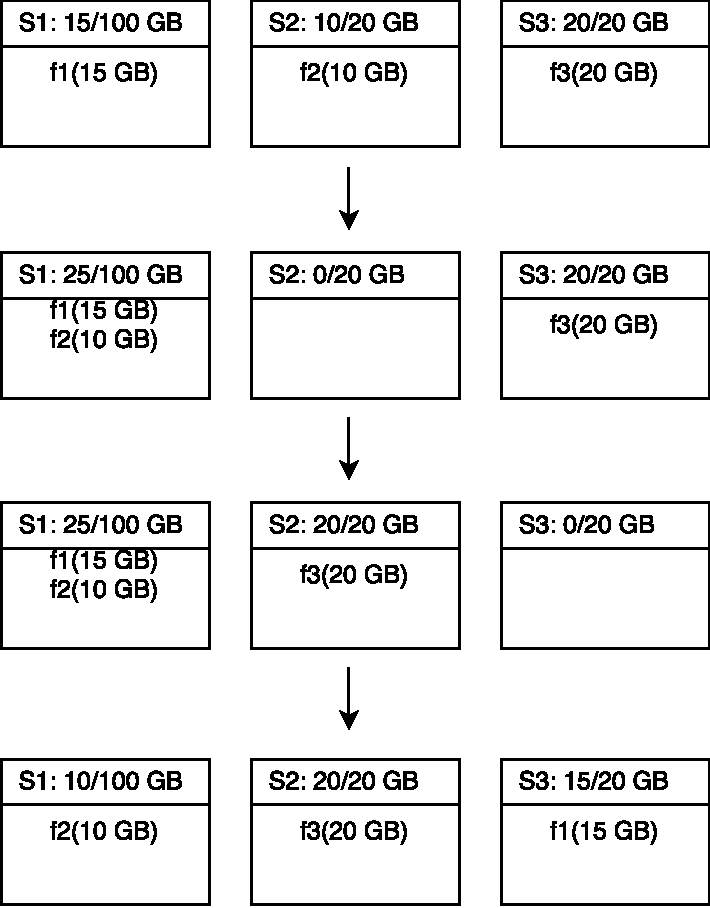
\includegraphics[width=80mm]{img/hie_migrace.pdf}
\caption{Příklad rozmístění souborů v hierarchickém systému}
\label{fig:hie_migrace}
\end{figure}

Na obr. \ref{fig:hie_migrace} máme 3 disky \textit{S1}, \textit{S2} a \textit{S3} seřazeny podle jejich rychlosti a chceme umístit soubor \textit{f1} o velikosti 15 GB na disk \textit{S3}. Výsledný proces migrace má celkem 3 kroky. Disk \textit{S3} má 0 GB volného prostoru, ale za předpokladu, že soubor \textit{f3} má nižší čítač přístupů než \textit{f1}, můžeme se pokusit odsunout \textit{f3} na disk \textit{S2}. Disk \textit{S2} nemá dostatek místa pro soubor \textit{f3}, ale po odsunutí souboru \textit{f2} na úložiště \textit{S1} již ano, které má zároveň dostatek volného místa. V 1. kroku tedy umístíme soubor \textit{f2} na úložiště \textit{S1}. V kroku 2 můžeme z disku \textit{S3} přesunout soubor na \textit{S2}. Posledním krokem je přesunutí souboru \textit{f1} na nyní již prázdný disk \textit{S3}.

\subsection{Logování}

Pro poskytnutí detailnějšího průběhu simulace jsou zaznamenávány detaily vybraných událostí, jakými jsou např. výběr cesty pro přenos dat, migrace dat a dokončení simulace požadavku. Logovací objekt implementující rozhraní \textit{DfsSimulatorLogger} je předán simulátoru při startu simulace.

Výchozí implementací je \textit{DfsStringSimulatorLogger}, který události ukládá jako řetězec do interního seznamu. Seznam všech logovaných událostí lze získat metodou \textit{getMessages}.

\subsection{Vzorkování rychlosti}

Aby bylo možné po doběhnutí simulace analyzovat průběh přenosu dat, je při každém kroku simulátoru vzorkována aktuální rychlost přenosu dat daného požadavku. Vzorkování probíhá pomocí objektu, který implementuje rozhraní \textit{SimulationThroughputSampler}. 

\subsubsection*{Filtrování vzorků}

Výchozí implementací vzorkovače je \textit{FilteringThroughputSampler}, který se snaží minimalizovat počet záznamů dodatečným filtrováním hodnot. Filtrování probíhá na základě porovnání předchozí vzorkované hodnoty s novou a pokud se rovnají, tak je nová hodnota zanedbána. Pokud by bylo žádoucí ještě více zmenšit počet vzorků, lze využít např. hranice minimálního rozdílu, o kterou se musí nový vzorek lišit či jiné pokročilé metody filtrování.

\section{Import a export prostředí}

Modul perzistence v balíku \textit{persistence} slouží k uložení modelovaného systému a simulačního plánu vybraného klienta. Třída, která chce být exportovatelná a následně obnovitelná musí implementovat rozhraní \textit{StatePersistable}. Export probíhá od kořenového prvku přes všechny jeho následníky.

\subsection{Elementy a atributy}

Exportují se dva typy objektů a to elementy \textit{StatePersistableElement} a atributy \textit{StatePersistableAttribute}. Atributem je jednoduchý objekt, který uchovává klíč (název atributu) a hodnotu. Element může mít atributy a další elementy jako následníky. Každý exportovaný objekt \textit{StatePersistable} je exportován jako element a své potomky může exportovat manuálně vytvořením objektů typu \textit{StatePersistableElement} a nebo vrácením seznamu potomků implementujících rozhraní \textit{StatePersistable} v metodě \textit{getPersistableChildren}. 

\subsection{Uložení stavu}

Uložení stavu simulátoru umožňuje objekt implementující rozhraní \textit{StatePersistor} metodou \textit{persist}, které se předá kořenový element. Každá třída implementující rozhraní \textit{StatePersistable} si řídí, jaké atributy a elementy budou součástí exportu. 

V metodě \textit{export}, která je rekurzivně volána od kořene, vrací \textit{StatePersistableElement}, kterému může nastavit atributy metodou \textit{addAttribute} a následníky metodou \textit{addElement}. Následníci, které třída vrací v metodě  \textit{getPersistableChildren} budou rekurzivně exportováni stejným způsobem, dokud se nenarazí na následníka, který žádné další následníky nemá.

\subsubsection*{Uložení do XML}

Výchozí implementací je \textit{FileXmlStatePersistor}, který nejprve exportuje stav do formátu XML a následně ho uloží do souboru. XML soubor je vytvořen pomocí knihoven z balíku \textit{javax.xml}, které jsou součástí výchozí instalace Javy.

\subsection{Načtení stavu}

Načtení stavu probíhá obdobně jako uložení. Řízení obnovení stavu má na starosti objekt implementující rozhraní \textit{StateRestorer} metodou \textit{restore}. Každá třída implementující rozhraní \textit{StatePersistable} si řídí obnovení svých atributů a potomků. 

Obnovení objektu probíhá zavoláním metody \textit{restoreState}, u které je jedním z parametrů aktuální element \textit{StatePersistableElement}, ze kterého lze získat všechny atributy elementu a jeho následníky. Element při obnově svých následníků volá opět metodu \textit{restoreState}.

\subsubsection*{Načtení z XML}

K třídě, která ukládá stav do XML je implementována třída \textit{FileXmlStateRestorer}, která tento uložený stav umožňuje obnovit. Obnova probíhá zavoláním metody \textit{restore}, která dostává jako parametr soubor s uloženým stavem.

\chapter{Implementace grafického rozhraní}

Soubory grafického rozhraní jsou rozděleny na dvě části, jednou je balík \textit{cz.zcu.kiv.dfs\_simulator.view}, který obsahuje veškerou logiku spojenou s GUI a druhou je adresář \textit{src/main/resources}, ve kterém jsou CSS\footnote{https://www.w3.org/Style/CSS/Overview.en.html} soubory, obrázky a FXML soubory popisující rozmístění grafických komponent.

\section{Rozložení GUI}

\begin{figure}[H]
\centering
	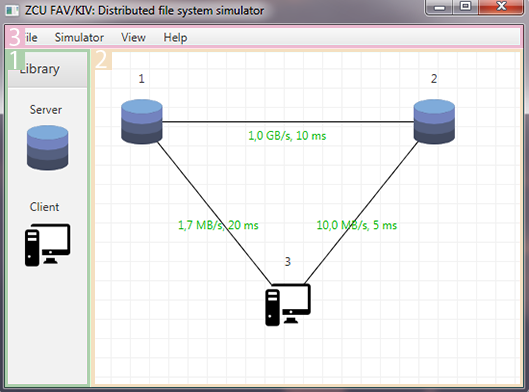
\includegraphics{img/rozlozeni_alt.png}
\caption{Rozložení grafických částí simulátoru}
\label{fig:gui_rozlozeni}
\end{figure}

Na obrázku \ref{fig:gui_rozlozeni} je vidět základní rozložení simulátoru, které se skládá ze tří částí a to: postranní panel s komponentami (1), plochou pro modelování systému (2) a horní menu (3). Všechny tyto části jsou součástí \textit{SimulatorLayoutPane}, které řeší jejich inicializaci a zprostředkovává jejich komunikaci pomocí událostí.

\section{Grafické komponenty}

Pro modelování systému jsou součástí GUI grafické komponenty, které jsou nadstavbou komponent modelu. Všechny grafické komponenty dědí od některého potomka \textit{javafx.Scene.Node}.

\subsection{Grafické uzly}

Hlavní grafickou komponentou je abstraktní třída \textit{FxModelNode}, která představuje uzel grafu a společnou grafickou logiku pro klient a server. Nadstavbou klienta je \textit{FxModelClientNode} a serveru \textit{FxModelServerNode}. Součástí grafického uzlu je i speciální textové pole \textit{FxModelNodeLabel}, které zobrazuje identifikátor uzlu.

\subsection{Grafická hrana}

Grafické propojení mezi uzly je řešeno pomocí třídy \textit{FxNodeConnectionWrapper}, která obaluje grafický prvek zobrazující propoj mezi uzly, dvě instance spojení \textit{ModelNodeConnection} a jednu společnou charakteristiku spoje \textit{LineConnectionCharacteristic}.

Tato obalová třída vyžaduje v konstruktoru mimo jiné zdrojový a cílový uzel a propustnost spoje. Přestože model umožňuje nesymetrické propoje, tedy různé vlastnosti spoje závislé na směru, grafická nadstavba aktuálně pracuje pouze se symetrickými spoji.
 
Viditelná hrana je na plátnu reprezentována třídou dědící od abstraktní třídy \textit{FxNodeLink}. Hrana může mít vlastní popisek a kontextové menu pro nastavení vlastností spoje. V základní verzi simulátoru jsou dvě třídy umožňující vykreslení hrany a to propojení úsečkou \textit{LineFxNodeLink} nebo Bézierovo křivkou \textit{BezierFxNodeLink}.

\section{Plátno pro modelování}

Modelování systému probíhá na plátně realizovaném pomocí \textit{ModelGraphLayoutPane}, které dědí od rodičovské třídy \textit{ScrollPane}. Rodičovská třída \textit{ScrollPane} umožní automatické rozšiřování plátna vytvořením nové komponenty či přesunutím stávající mimo pravý nebo dolní okraj plátna.

Plátno akceptuje události vyvolané upuštěním komponenty z knihovny a reaguje na ně vytvořením odpovídající komponenty na plátně se souřadnicemi získanými z kurzoru myši. Mimo tyto události ještě slouží pro odchytávání událostí vyvolaných komponentami na plátně, a to události jako je vytvoření hrany mezi uzly či otevření konfiguračního dialogu komponenty. Reakce na události jsou registrovány v metodě \textit{setActionEventHandlers}.

\section{Přesun komponent myší}

Některé komponenty ležící plátně reagují na události vyvolané tažením myši aktualizací své pozice podle pozice kurzoru myši. Logika přesunu komponenty je předána metodě \textit{setOnMouseDragged} dostupné z rodičovské třídy. 

Ještě před tažením myši je zaregistrována událost kliknutí myší na komponentu, během které si komponenta interně uloží rozdíl pozice kurzoru od svého levého horního rohu. Rozdíl pozice kurzoru je uložen aby bylo možné správně vypočítat nové souřadnice komponenty na základě aktualizované pozice kurzoru.

V případě grafického uzlu je ještě před aktualizací pozice v metodě \textit{handleNodeDragged} ověřeno, zda nové souřadnice neleží mimo plátno. Pokud je vše v pořádku, komponenta aktualizuje svojí pozici metodami \textit{setLayoutX} a \textit{setLayoutY}.

\subsection{Výběr více komponent}

\begin{figure}
\centering
	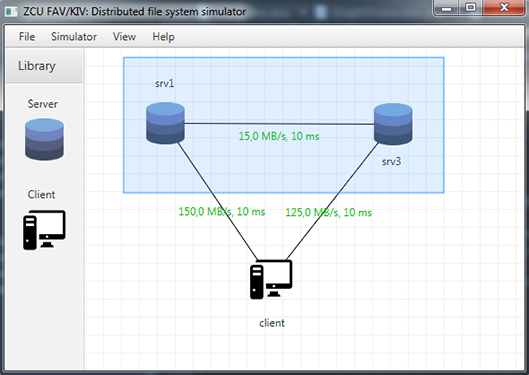
\includegraphics{img/multi_selekce.png}
\caption{Výběr více komponent najednou}
\label{fig:selekce_najednou}
\end{figure}

Aby bylo možné komponentu vybrat spolu s jinými komponentami, musí implementovat rozhraní \textit{MultiSelectableDraggable}. Vybrání více komponent probíhá tažením obdélníku z některého bodu plátna a všechny komponenty nacházející se vně tohoto obdélníku jsou označeny najednou (viz obr. \ref{fig:selekce_najednou}).

Výběr více komponent zařizuje třída \textit{RubberBandSelection}, která v konstruktoru dostane instanci plátna pro modelování \textit{ModelGraphLayoutPane}. Do předané instance vloží své handlery událostí vyvolané myší, kterými se výběr vytváří. Po dokončení výběru projde všechny potomky uvnitř výběru, kteří implementují rozhraní \textit{MultiSelectableDraggable} a přidá je do výběru.

Každá komponenta je notifikována metodou \textit{setMultiSelectableState}, zda se nachází ve vícenásobném výběru komponent a tento stav si interně uloží. Komponenta poté v handleru \textit{setOnMouseDragged} na základě stavu může notifikovat ostatní komponenty ve výběru vyvoláním události \textit{MultiNodeSelectionEvent}, konkrétně typu \textit{DRAG\_SELECTION}.

\section{Konfigurace komponenty}

Komponenty typu uzel a linka mohou být dodatečně konfigurovány. Konfigurace probíhá přes kontextové menu vyvoláním konfiguračního dialogu pro danou komponentu.

\subsection{Konfigurace serveru}

\begin{figure}
\centering
	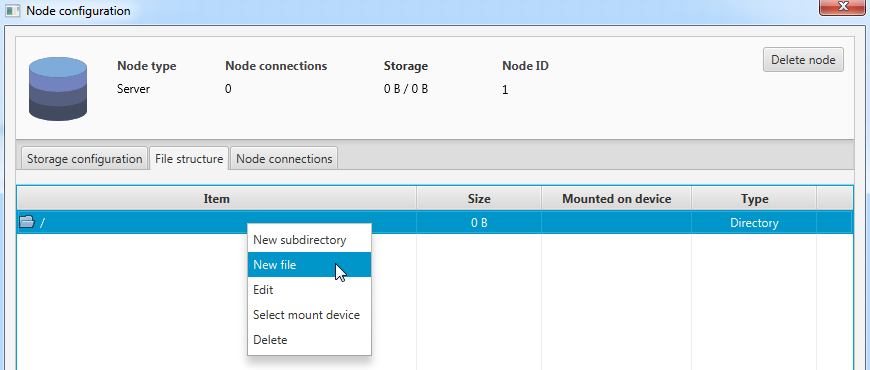
\includegraphics[width=\textwidth]{img/konfig_server.png}
\caption{Dialog konfigurace serveru - adresářová struktura}
\label{fig:server_konfigurace}
\end{figure}

Konfigurace serveru probíhá pomocí dialogu \textit{FxServerNodeContextDialog}. Dialog je rozdělen na záložky a umožňuje konfigurovat úložiště, adresářovou strukturu a spojení s ostatními uzly. Konfigurace úložiště probíhá pomocí tabulky \textit{FxStorageTable}, která zobrazuje aktuální úložiště serveru a pomocí kontextového menu s ním lze dále pracovat (viz obr. \ref{fig:server_konfigurace}).

\subsubsection*{Vytváření adresářové struktury}

Adresářová struktura serveru je přístupná pomocí tabulky se stromovou strukturou \textit{FxFsTable}. Tabulka přes kontextové menu umožňuje vytváření adresářů, souborů a nastavení úložiště, na kterém se složka nebo soubor nachází. 

Vytvoření adresáře probíhá přes jednoduchý dialog \textit{FxFsDirectoryDialog}, ve kterém stačí specifikovat název nové složky. Rodičem složky bude složka z odpovídající úrovně stromové struktury, ze které bylo vyvoláno kontextové menu.

\begin{figure}
\centering
	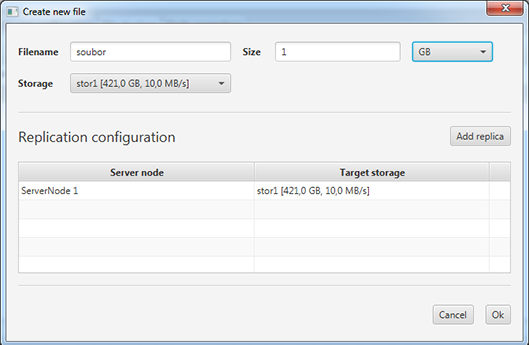
\includegraphics{img/vytvareni_soubor.png}
\caption{Dialog pro vytvoření a úpravu souboru}
\label{fig:vytvareni_soubor}
\end{figure}

Vytváření a úpravu souborů umožňuje dialog \textit{FxFsFileDialog} (obr. \ref{fig:vytvareni_soubor}), který vyžaduje jméno souboru, velikost a úložiště. Při vytváření lze specifikovat i repliky souboru, které budou automaticky vytvořeny na odpovídajících serverech a vybraných úložištích. Při replikaci souboru je nejdřív zkontrolováno, zda je na všech úložištích dostatek místa pro soubor ve třídě \textit{FsGlobalReplicationManager} metodou \textit{updateReplicaTargets}. Není-li dostatek místa, je vyvolána vyjímka \textit{NotEnoughSpaceLeftException}, která je zachycena a pomocí dialogu je uživateli umožněno automaticky místo rozšířit.

\subsection{Konfigurace klienta}

Konfigurace klienta probíhá dialogem \textit{FxClientNodeContextDialog} na podobném principu jako při konfiguraci serveru. Dialog je rozdělen na dvě záložky kde v jedné je konfigurace simulačního plánu a v druhé tabulka s spojení s ostatními uzly. V záložce simulační plán lze rovněž vybrat jeden nebo více typů simulace, odstartovat simulaci podle simulačního plánu a následně spustit její vizualizaci vyvoláním události \textit{FxNodeSimulationEvent} typu \textit{SIMULATION\_VISUALISATION\_ON\_REQUESTED}, kterou zachytí \textit{SimulatorLayoutPane}.

\subsection{Konfigurace spojení}

Dialog \textit{FxNodeLinkDialog} slouží k vytvoření nového spojení a konfiguraci existujícího. U spojení umožňuje konfigurovat jeho rychlost a latenci. Další možností konfigurace existujícího spojení je úprava jeho zátěžové charakteristiky, která probíhá vyvoláním dialogu \textit{FxNodeLinkCharacteristicDialog} přes kontextové menu spojení. 

\begin{figure}
\centering
	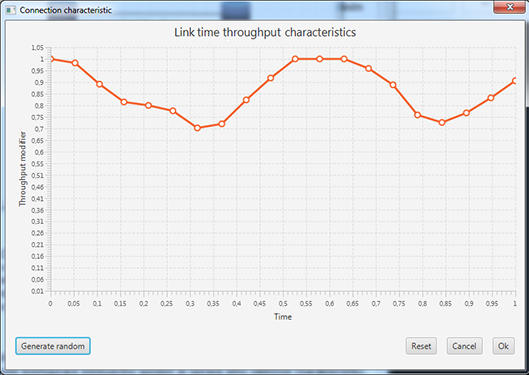
\includegraphics{img/zatezova_charakteristika.png}
\caption{Zátěžová charakteristika spojení}
\label{fig:zatezova_charakteristika}
\end{figure}

Konfigurace lineární zátěžové charakteristiky probíhá pomocí spojnicového grafu, který vykresluje diskrétní body  charakteristiky a spojnice mezi nimi (obr. \ref{fig:zatezova_charakteristika}). Body grafu, jejichž chování je řízeno třídou \textit{MarkerNodeMoveHandler}, lze posouvat myší podél osy $y$ udávající modifikátor propustnosti v daném čase.

\section{Průběh simulace a její vizualizace}

Spuštění simulace probíhá nastavení konkrétního klienta. Klient může vybrat jeden nebo více typů simulace (\textit{SimulationType}), které budou simulovány a vytvořit seznam simulovaných požadavků. Při vybrání více typů simulace proběhne simulace opakovaně pro každý typ zvlášť se stejnými simulovanými požadavky. Simulované požadavky jsou provedeny opakovaně pro každý typ simulace. Po spuštění simulace je zobrazen dialog s progress barem, který indikuje kolik typů simulací ještě zbývá provést. Během simulace jsou výsledky simulace akumulovány v seznamu, který je následně předán do \textit{SimulatorLayoutPane} pomocí události \textit{FxNodeSimulationEvent}.

\begin{figure}
\centering
	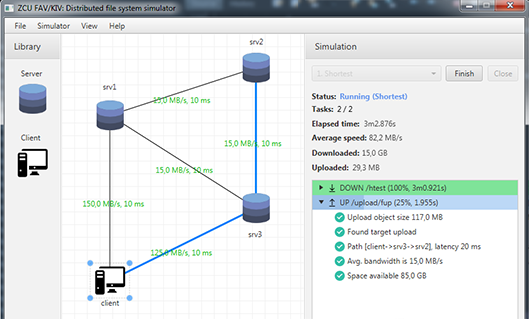
\includegraphics{img/vizualizace_simulace.png}
\caption{Vizualizace simulace}
\label{fig:vizualizace_simulace}
\end{figure}

Průběh simulace je rekonstruován z výsledků a zrychleně přehrán uživateli objektem třídy \textit{FxSimulationPlayer}. Podoba vizualizace je zobrazena na obrázku \ref{fig:vizualizace_simulace}. Na plátně pro modelování lze vidět zvýrazněnou cestu modrou barvou od klienta k cílovému serveru a v pravé části průběh simulace požadavků.

\subsection{Zvýraznění cesty}

Při vizualizaci jsou pro každý požadavek zvýrazněny všechny cesty, kudy tekla data od klienta k serveru (replikace není zohledněna). Během simulace je ukládána historie cest u každého požadavku (viz \ref{vysledkypozadavku}). Všechny unikátní hrany z historie jsou sjednoceny do množiny \textit{FxNodeLink}, pro kterou je nad každým prvkem zavolána metoda

\begin{verbatim}
void setLinkHighlighted(boolean highlighted),
\end{verbatim}
\noindent kde parametr \textit{highlighted} udává, zda má být zvýraznění zapnuto či vypnuto.

\subsection{Průběh požadavků}

Rozhraní \textit{SimulationLogDisplayable} popisuje metody, které musí být implementovány pro simulaci průběhu požadavků. Základní implementací je \textit{FxSimulationBar}, který tvoří postranní panel se seznamem proběhlých typů simulací a aktuálním pohledem na simulované požadavky.

Seznam požadavků je zobrazen pomocí objektu třídy \textit{TreeView}. Každý požadavek tvoří vrchol stromu a může mít libovolné následníky, poskytující dodatečné stavové informace. Přidání vrcholu do stromu požadavků probíhá metodou 

\begin{verbatim}
void logSimulationEvent(FxSimulationLogEvent event),
\end{verbatim}
\noindent která může pomocí parametru \textit{event} specifikovat svého předchůdce. Vizualizace umožňuje vykreslit maximálně dvě úrovně, kde první úrovní jsou požadavky a druhou úrovní jsou stavové informace přiřazené k požadavkům. Stávající vrcholy lze aktualizovat metodou \textit{updateSimulationEvent}.

\subsubsection*{Animace průběhu}

Během vizualizace průběhu požadavku je periodicky měněna CSS třída pozadí vrcholu požadavku. Pozadí požadavku vizualizuje procentuální průběh a je implementováno pomocí třídy \textit{PseudoClass}, která umožňuje dynamickou změnu aktivních CSS tříd elementu. Změna pozadí probíhá v metodě \textit{updateCellPseudoClass} po každé aktualizaci vrcholu.

\section{Výsledky simulace}

\begin{figure}[H]
\centering
	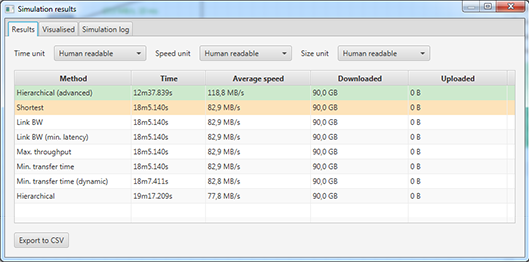
\includegraphics{img/vysledky_simulace.png}
\caption{Okno s výsledky simulace}
\label{fig:vysledky_simulace}
\end{figure}

Pro zobrazení výsledků slouží okno \textit{SimulationResultsWindow}. Ve výsledcích jsou tři záložky a to souhrnné výsledky, graf průběhu rychlosti a detailní log průběhu simulace (viz obr. \ref{fig:vysledky_simulace}). 

V tabulce se souhrnnými výsledky jsou pomocí změny CSS třídy zvýrazněny dva nejlepší výsledky. Změnou volby v jednom ze seznamů \textit{ChoiceBox} pro výběr násobků je vyvolána aktualizace, která pomocí metod \textit{getConvertedResultTime}, \textit{getConvertedResultSize} a \textit{getConvertedResultSpeed} získá přepočtené hodnoty měření a následně je vykreslí.

\subsection{Graf průběhu rychlosti}

\begin{figure}
\centering
	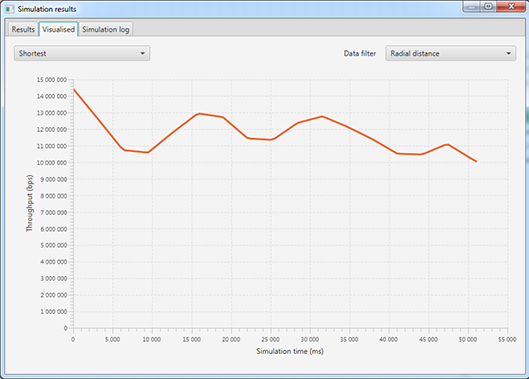
\includegraphics{img/graf_rychlost_simulace.png}
\caption{Graf průběhu rychlosti}
\label{fig:graf_rychlost_simulace}
\end{figure}

Na obrázku \ref{fig:graf_rychlost_simulace} je vidět graf \textit{LineChart} zobrazující průběh rychlosti simulace v závislosti na čase. Průběh rychlosti v grafu je složen ze všech simulovaných požadavků. 

\subsection{Filtrace vzorků rychlosti} \label{filtracevzorku}

Navzorkovaných hodnot rychlosti během simulace bývá mnoho a jejich vykreslení je poměrně náročné. Z tohoto důvodu jsou vytvořeny filtry hodnot grafu, které se snaží odstranit vzorky, jejichž odebrání nebude mít zásadní vliv na podobu grafu. Filtr musí implementovat rozhraní \textit{SimulationThroughputHistoryReducer}, kde metodou

\begin{verbatim}
List<Pair<Long, Long>> reduce(
    List<Pair<Long, Long>> original, 
    long totalElapsedTime, 
    ByteSpeed totalAverageSpeed)
\end{verbatim}
\noindent vrací redukovaný seznam původních hodnot v seznamu \textit{original}. Implementovanými filtry jsou

\begin{itemize}
\item \textbf{AllInclusiveThroughputHistoryReducer} vrací všechny vzorky, náročný, přesný ale ne příliš vhodný pokud máme hodně vzorků.
\item \textbf{DouglasPeuckerThroughputHistoryReducer} využívá Douglas-Peucker algoritmu \cite{douglaspeuckeralg}.
\item \textbf{RadialDistanceThroughputHistoryReducer} funguje na bázi eukleidovské vzdálenosti bodů.
\item \textbf{MovingAverageReducer} výchozí filtr - dělí hodnoty do časových intervalů a pro každý časový interval počítá průměr hodnot. Filtrace probíhá rychle i pro větší množství vzorků.
\end{itemize}

\chapter{Testy} \label{testy}

V této kapitole jsou popsány provedené testy pro ověření programové funkčnosti simulátoru a měření navrhovaného distribuovaného souborového systému s hierarchickým modelem uložení dat. Model a plán simulace vycházejí z výzkumu Ing. Pešičky a slouží pro ověření vlastností navrhovaného modelu.

\section{Unit testy} \label{unittesty}

Pro ověření základní funkčnosti simulátoru byly vytvořeny unit testy, které pokrývají nejdůležitější funkčnost aplikační části simulátoru. Testy jsou umístěny ve složce \textit{src/test}. V následujících kapitolách budou zmíněny testy nejdůležitější funkcionality. Uváděné názvy balíku jsou vždy relativní cestou k výchozímu balíku \textit{cz.zcu.kiv.dfs\_simulator}.

\subsection{Testy spojení}

Spojení mezi uzly je testována uvnitř balíku \textit{model.connection} a to třemi třídami \textit{ModelNodeConnectionTest}, \textit{ModelNodeConnectionManagerTest} a \textit{LineConnectionCharacteristicTest}.

\subsubsection*{ModelNodeConnectionTest}

Uvnitř testovací třídy \textit{ModelNodeConnectionTest} je testována základní funkčnost třídy \textit{ModelNodeConnection}. Test ověřuje vytvoření spojení mezi dvěma uzly, správný počáteční a cílový uzel (test orientace spojení), hodnotu maximální propustnosti spojení a výpočet průměrné přenosové rychlosti během specifikovaného času.

\subsubsection*{ModelNodeConnectionManagerTest}

Tato testovací třída testuje funkcionalitu \textit{ModelNodeConnectionManager} a to konkrétně vytvoření obousměrného spojení mezi uzly, získání přímých sousedů uzlů a získání všech dostupných uzlů z výchozího uzlu.

\subsubsection*{LineConnectionCharacteristicTest}

Cílem této testovací třídy je ověřit funkcionalitu lineární periodické charakteristiky \textit{LineConnectionCharacteristic} a jejího vlivu na propustnost spojení mezi uzly. Během testu je nejdříve otestována propustnost linky v čase, ve kterém je přímo definována charakteristika, následně je otestována propustnost v čase ležící mimo definované body a nakonec průměrná propustnost během celého intervalu. Hodnoty charakteristiky jsou porovnávány s hodnotami vypočtenými podle vzorce uvedeného u lineární zátěžové charakteristiky v kapitole \ref{zatezovacharakteristika}.

\subsection{Testy souborového systému}

Následující testy v balíku \textit{model.storage.filesystem} slouží pro ověření funkčnosti spojené se souborovým systémem.

\subsubsection*{FsDirectoryTest}

Testovací třída \textit{FsDirectoryTest} ověřuje základní funkcionalitu spojenou s třídou \textit{FsDirectory}. Hlavním cílem je testování správného vytváření cesty přes všechny potomky až ke kořeni, vyhledávání přímo v dané složce a vyhledávání v některém z potomků složky (vnořená složka) a vyhledání potomka podle cesty a typu (soubor či složka).

\subsubsection*{FsFileTest}

Tato třída testuje funkčnost třídy \textit{FsFile} a to získání absolutní cesty k souboru přes všechny jeho předchůdce až ke kořenové složce, získání velikosti souboru a nastavení nové velikosti souboru a funkčnost čítače přístupů k souboru.

\subsubsection*{FsObjectChildContainerTest}

Uvnitř této třídy je testována třída \textit{FsObjectChildContainer}, která slouží k výpočtu velikosti všech potomků a výpočtu velikosti všech potomků, kteří nejsou explicitně umístěni na některém úložišti (tedy budou sdílet úložiště rodiče).

\subsubsection*{ServerFsManagerTest}

Cílem této třídy je otestovat funkcionalitu třídy \textit{ServerFsManager}, která slouží ke správě souborového systému serveru. Uvnitř testovací třídy je testováno zjištění velikosti obsazeného místa na daném úložišti, úspěšné přidání potomka do složky a neúspěch při přidání potomka do složky, které by způsobilo nedostatek místa na úložišti. Dále je testováno umístění souboru na úložiště, zjištění, na kterém úložišti je soubor uložen a zda se může soubor zvětšit na danou velikost aniž by přesáhl limit dostupného místa na úložišti.

\subsection{Testy diskových operací}

Testy v balíku \textit{model.storage} testují diskové operace probíhající na úložišti.

\subsubsection*{StorageOperationManagerTest}

Třída \textit{StorageOperationManagerTest} testuje správce diskových operací \textit{StorageOperationManager}. V této testovací třídě je ověřováno správné vytvoření diskových operací, dělení rychlosti mezi běžící operace a výpočet přenesených dat pro každou operaci za danou dobu.

\subsection{Testy vyhledávání cesty a metrik}

Testy, které ověřují výpočet metriky cesty, jsou v balíku \textit{model.simulation.path} a testy vyhledávání podle vypočtených metrik v \textit{model.simulation.graph.metric}.

\subsubsection*{Testování výpočtu metriky cesty}

Testy metriky testují správný výpočet metriky pro danou cestu. V následujícím seznamu je uveden seznam testovacích tříd a metrik, které testují:

\begin{itemize}
\item \textbf{DistanceMetricTest} testuje třídu \textit{DistanceMetrik} a kontroluje ohodnocení nejkratší cesty,
\item \textbf{LinkBwMetricTest} testuje třídu \textit{LinkBwMetric} a kontroluje ohodnocení cesty s maximální propustností spojení,
\item \textbf{LinkBwLatencyMetricTest} testuje třídu \textit{LinkBwLatencyMetric} a kontroluje ohodnocení cesty s maximální propustností spojení a minimální latencí,
\item \textbf{PathThroughputMetricTest} testuje třídu \textit{PathThroughputMetric} a kontroluje ohodnocení cesty s maximální propustností spojení a maximální rychlostí disku,
\item \textbf{PathThroughputLatencyMetricTest} testuje třídu \textit{PathThroughputLatencyMetric} a kontroluje ohodnocení cesty s maximální propustností spojení, maximální rychlostí disku a minimální celkové latenci,
\item \textbf{HierarchicalThroughputMetricTest} testuje třídu \textit{HierarchicalThroughputMetric} a kontroluje správné určení maximální rychlosti disku, pokud by byla provedena migrace.
\end{itemize}

\subsubsection*{MetricDfsPathPickerTest}

Tato testovací třída testuje třídu \textit{MetricDfsPathPicker}, konkrétně nalezení odpovídající cesty podle použité metriky.

\subsection{Testy simulace}

V balíku \textit{model.simulation} je testována funkčnost simulace.

\subsubsection*{DfsTimeSliceSimulatorTest}

V této testovací třídě je testován simulátor \textit{DfsTimeSliceSimulator}. Během testu je ověřeno správné stažení souboru, nahrání souboru, ověření úspěšného zapsání souboru na cílový server a simulace přenosu dat přes zatíženou linku konstantním modifikátorem propustnosti.

\subsubsection*{DfsSimulatorSimulationResultTest}

Tato třída testuje třídu \textit{DfsSimulatorSimulationResult}, která reprezentuje výsledky běhu simulace. Na třídě je testováno zejména výpočet souhrnných ukazatelů simulace jako je celkový čas, průměrná rychlost a celkový počet přenesených dat.

\section{Model distribuovaného souborového systému}

\begin{figure}
\centering
	\fbox{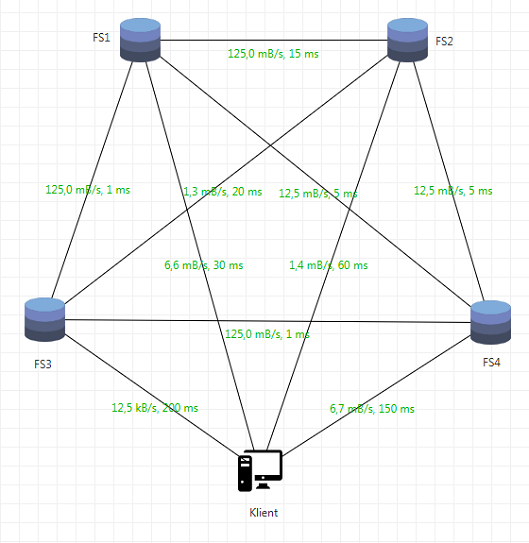
\includegraphics{img/test/model.png}}
\caption{Testovaný model distribuovaného souborového systému}
\label{fig:test_model}
\end{figure}

Na obrázku \ref{fig:test_model} lze vidět vybraný model distribuovaného souborového systému, který se skládá ze 4 datových serverů (FS1-FS4) a 1 klienta. Popisek spojení udávající propustnost a latenci je vždy zhruba uprostřed úsečky spojující uzly. Každý uzel modelu je propojen se všemi ostatními, jedná se tedy o úplný graf (viz překryvná síť v kapitole \ref{vybercesty}) a vlastnosti hran jsou zaznamenány v tabulce \ref{table:uzlyspojeni}. Použitý model distribuovaného souborového systému lze najít na přiloženém CD v souboru \textit{prostredi/configuration.xml}.

\begin{table}
\centering
\caption{Spojení mezi uzly}
\label{table:uzlyspojeni}
\begin{adjustbox}{max width=\textwidth}
\begin{tabular}{|l|l|l|l|l|l|}
\hline
\textbf{}       & \textbf{FS1}   & \textbf{FS2}   & \textbf{FS3}     & \textbf{FS4}     & \textbf{Klient}   \\ \hline
\textbf{FS1}    & -              & 125 mB/s, 15ms & 125 mB/s, 1ms    & 12,5 mB/s, 5ms   & 6,6 mB/s, 30ms    \\ \hline
\textbf{FS2}    & 125 mB/s, 15ms & -              & 1,3 mB/s, 20ms   & 12,5 mB/s, 5ms   & 1,4 mB/s, 60ms    \\ \hline
\textbf{FS3}    & 125 mB/s, 1ms  & 1,3 mB/s, 20ms & -                & 125 mB/s, 1ms    & 12,5 kB/s, 200 ms \\ \hline
\textbf{FS4}    & 12,5 mB/s, 5ms & 12,5 mB/s, 5ms & 125 mB/s, 1ms    & -                & 6,7 mB/s, 150 ms*  \\ \hline
\textbf{Klient} & 6,6 mB/s, 30ms & 1,4 mB/s, 60ms & 12,5 kB/s, 200ms & 6,7 mB/s, 150 ms* & -                 \\ \hline
\end{tabular}
\end{adjustbox}
\raggedright{* Spojení je zatíženo podle charakteristiky v \ref{testzatizenispojeni}.}
\end{table}

\subsection{Testovací prostředí}

Simulace proběhla na počítači s procesorem \textit{i5 4670k@4.3 GHz}, \textit{16 GB RAM@2133 MHz}, úložištěm \textit{Samsung SSD 840 EVO} a operačním systémem \textit{MS Windows 7}. Jako virtuální stroj javy byl použit \textit{Java HotSpot(TM) 64-Bit Server VM (build 25.111-b14, mixed mode)} s parametry \textit{-Xmx4g -Xms4g}. 

\subsection{Zatížení spojení}\label{testzatizenispojeni}

\begin{figure}
\centering
	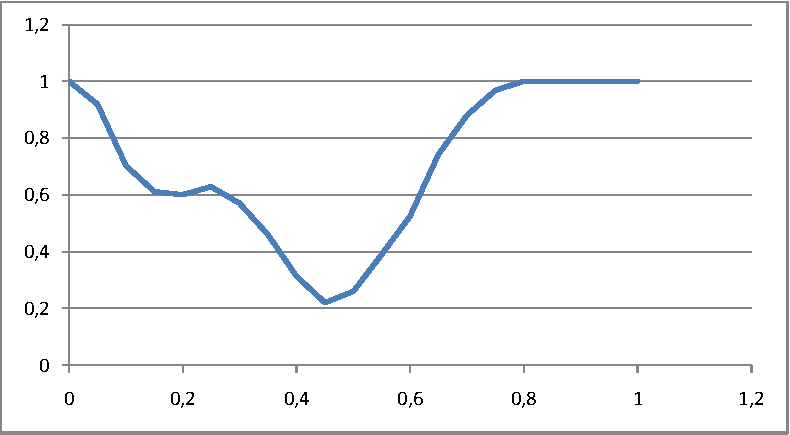
\includegraphics[width=100mm]{img/test/zatizeni.pdf}
\caption{Zatížení spojení FS4 -> klient}
\label{fig:test_zatizeni_spojeni}
\end{figure}

\begin{table}[]
\small
\centering
\caption{Hodnoty bodů definujících lineární zátěžovou charakteristiku}
\label{table:test_body_charakteristiky}
\begin{tabular}{|l|l|}
\hline
\textbf{Čas} & \textbf{Modifikátor propustnosti} \\ \hline
0            & 1                                 \\ \hline
0.05         & 0,918539325842696                 \\ \hline
0.1          & 0,702359551                       \\ \hline
0.15         & 0,611797753                       \\ \hline
0.2          & 0,60011236                        \\ \hline
0.25         & 0,629325843                       \\ \hline
0.3          & 0,570898876                       \\ \hline
0.35         & 0,45988764                        \\ \hline
0.4          & 0,313820225                       \\ \hline
0.45         & 0,220337079                       \\ \hline
0.5          & 0,261235955                       \\ \hline
\end{tabular}
\begin{tabular}{|l|l|}
\hline
\textbf{Čas} & \textbf{Modifikátor propustnosti} \\ \hline
0.55         & 0,389775281                       \\ \hline
0.6          & 0,524157303                       \\ \hline
0.65         & 0,743258427                       \\ \hline
0.7          & 0,880561798                       \\ \hline
0.75         & 0,968202247                       \\ \hline
0.8          & 1                                 \\ \hline
0.85         & 1                                 \\ \hline
0.9          & 1                                 \\ \hline
0.95         & 1                                 \\ \hline
1            & 1                                 \\ \hline
\end{tabular}
\end{table}

Spojení mezi serverem $FS4$ a klientem bylo zatíženo periodickou lineární charakteristikou s periodou 60 sekund. Konkrétní hodnoty charakteristiky byly náhodně vygenerovány. Průběh charakteristiky lze vidět na obrázku \ref{fig:test_zatizeni_spojeni} a detailněji popsán v tabulce \ref{table:test_body_charakteristiky} hodnotami diskrétních bodů definujících zátěžovou charakteristiku. 

Čas charakteristiky je definován na intervalu $<0, 1>$ a pro získání simulačního času z tabulky je hodnota času vynásobena délkou periody, tedy např. čas $0.1$ po vynásobení délkou periody $0.1 * 60s$ odpovídá zátěži v simulačním čase $6s$, v další periodě zase $66s$ a takto se opakuje až do konce simulace. Modifikátor propustnosti ovlivňuje propustnost spojení v odpovídajícím čase a výsledná propustnost je výsledkem vynásobení maximální propustností spojení definovaným modifikátorem. Ostatní spoje mají konstantní propustnost rovnou jejich maximální propustnosti. 

\subsection{Simulovaná data a úložiště}

V distribuovaném souboru jsou celkem 4 soubory: \textit{f1}, \textit{f2}, \textit{f3} a \textit{f4}. Číslování souborů odpovídá názvům serverů. Jediný soubor \textit{f4} je replikován a to na server \textit{FS1} a \textit{FS4}. Dva servery (\textit{FS1} a \textit{FS4}) mají dvě různá úložiště a lze na nich vyzkoušet hierarchické migrace dat. Parametry úložišť a rozmístění souborů lze vidět v tabulce \ref{table:test_data_uloziste}

\begin{table}[]
\centering
\caption{Rozmístění souborů na jednotlivá úložiště}
\label{table:test_data_uloziste}
\begin{tabular}{|l|l|l|}
\hline
\textbf{Server} & \textbf{Úložiště}             & \textbf{Soubory} \\ \hline
\textbf{FS1}    & STOR10 {[}100 mB, 1 gB/s{]}   &                  \\ \hline
                & STOR11 {[}10 TB, 5 mB/s{]}    & f1 [15 mB], f4 [450 mB]            \\ \hline
\textbf{FS2}    & STOR20 {[}250 gB, 500 mB/s{]} & f2 [100 mB]              \\ \hline
\textbf{FS3}    & STOR30 {[}5 TB, 5 mB/s{]}     & f3 [4 mB]              \\ \hline
\textbf{FS4}    & STOR40 {[}5 TB, 5 mB/s{]}     & f4 [450 mB]              \\ \hline
                & STOR41 {[}1 TB, 200 mB/s{]}   &                  \\ \hline
\end{tabular}
\end{table}

\section{Testované modely}

Pro otestování simulátoru byly vybrány následující modely distribuovaného souborového systému a jejich strategie hledání cesty mezi klientem a serverem. 

V tabulce \ref{table:test_metody} jsou vyjmenované testované metody a jejich vlastnosti. Význam vlastností je:

\begin{itemize}
\item \textbf{Nejkr.} Metoda hledá nejkratší cestu (nejméně skoků), používána většinou existujících distribuovaných souborových systémů (viz \ref{vybercesty}).
\item \textbf{Max. prop.} Metoda hledá cestu s maximální propustností linek.
\item \textbf{Min. lat.} Metoda hledá cestu s nejmenší latencí.
\item \textbf{R. disk} Metoda hledá cestu s nejrychlejším diskem.
\item \textbf{D. rout.} Metoda využívá dynamického routování - metoda výběru cesty v KIVFS (viz \ref{vybercesty}).
\item \textbf{Hie.} Metoda využívá hierarchické migrace souborů na základě čítačů přístupů a k přesunu souborů používá strategii LFU pro uvolnění místa (\ref{planovac_lru}).
\item \textbf{H. adv.} Jako \textit{Hie.}, ovšem při výběru cesty bere za rychlost disku nejvyšší možnou vrstvu, na kterou by šel soubor z požadavku umístit. Experimentální metoda vycházející z výzkumu Ing. Pešičky.
\end{itemize}

\begin{table}[]
\centering
\caption{Testované metody}
\label{table:test_metody}
\begin{adjustbox}{max width=\textwidth}
\begin{tabular}{|l|l|l|l|l|l|l|l|}
\hline
\textbf{Metoda}                   & \textbf{Nejkr.} & \textbf{Max. prop.} & \textbf{Min. lat.} & \textbf{R. disk} & \textbf{D. rout.} & \textbf{Hie.} & \textbf{H. adv.} \\ \hline
\textbf{Shortest}                 & \checkmark                &                     &                    &                      &                     &               &              \\ \hline
\textbf{Link BW}                  &                 & \checkmark                   &                    &                      &                     &               &              \\ \hline
\textbf{Link BW (min. lat)}       &                 & \checkmark                  & \checkmark                  &                      &                     &               &              \\ \hline
\textbf{Max. throughput}          &                 & \checkmark                &                    & \checkmark                    &                     &               &              \\ \hline
\textbf{Min. tx time}       &                 & \checkmark                   & \checkmark                   & \checkmark                     &                     &               &              \\ \hline
\textbf{Min. tx time (dyn.)} &                 & \checkmark                   & \checkmark                 & \checkmark                     & \checkmark                    &               &              \\ \hline
\textbf{Hierarchical}             &                 & \checkmark                   & \checkmark                  & \checkmark                    & \checkmark                   & \checkmark             &              \\ \hline
\textbf{Hierarchical (adv.)}   &                 & \checkmark                   & \checkmark                & \checkmark                   & \checkmark                  & \checkmark             & \checkmark            \\ \hline
\end{tabular}
\end{adjustbox}
\end{table}

\section{Plán simulace}

Plán simulace je tvořen 1000 požadavky v náhodném pořadí pro každý soubor \textit{f1}, \textit{f2}, \textit{f3} a \textit{f4}. Celkem se tedy jedná o 4000 požadavků s celkovým přenosem 569 gB dat. Testovaný plán simulace je dostupný v příloze této práce v souboru \textit{prostredi/simulation-plan.xml}.

\section{Výsledky} 

V tabulce \ref{table:test_vysledky} jsou uvedeny výsledky simulace pro testované metody. Celkový čas simulace pro všech 8 testovaných metod byl \textit{47.53s} (samotná simulace bez vykreslení výsledků) a ve špičce bylo využito \textit{1.54 GB RAM} (měřeno profilerem \textit{Netbeans profiler} \cite{netbeansprofileronline}).

\begin{table}[]
\centering
\caption{Výsledky měření času běhu a rychlosti}
\label{table:test_vysledky}
\begin{tabular}{c|cc}
\hline
\textbf{Metoda}                   & \textbf{Čas přenosu} & \textbf{Průměrná rychlost} \\ \hline
\hline
\rowcolor{HoneyDew}
\textbf{Hierarchical (advanc.)}   & 26h 14m 9.899s     & 6.024 mB/s                 \\ \hline
\textbf{Hierarchical}             & 28h 37m 55.316s     & 5.088 mB/s                 \\ \hline
\textbf{Min. transf. time (dyn.)} & 36h 36m 46.061s     & 5.054 mB/s                  \\ \hline
\textbf{Max. throughput}          & 43h 49m 37.367s     & 4.865 mB/s                 \\ \hline
\textbf{Min. transfer time}       & 32h 29m 17.836s     & 4.865 mB/s                  \\ \hline
\textbf{Link BW (min. lat)}       & 39h 46m 57.808s     & 3.972 mB/s                  \\ \hline
\textbf{Link BW}                  & 40h 2m 14.388s     & 3.947 mB/s                  \\ \hline
\textbf{Shortest}                 & 134h 39m 8s         & 1.173 mB/s                 \\ \hline
\end{tabular}\end{table}

Nejpomalejší metodou testu byla metoda \textit{Shortest}, která hledá pouze nejkratší cestu. Nejrychlejší metodou byla \textit{Hierarchical (advanc.)}, která hledá cestu s nejvyšší maximální propustností, využívá dynamického routování a hierarchického modelu uložení dat.

V následující části jsou uvedeny tabulky s cestou pro jednotlivé soubory a zdůvodnění výsledků testovaných metod. V tabulce cest je uveden soubor a cesta přes všechny uzly, u které je zobrazena maximální přenosová rychlost (zohledněna maximální přenosová rychlost disku) a latence.

\subsection{Shortest}
\begin{table}[H]
\centering
\caption{Cesty metody Shortest}
\label{table:test_shortest_routy}
\begin{tabular}{|l|l|}
\hline
\textbf{Soubor} & \textbf{Cesta}           \\ \hline
f1              & Klient -> FS1 [5 mB/s, 30 ms] \\ \hline
f2              & Klient -> FS2 [1,4 mB/s, 60 ms]\\ \hline
f3              & Klient -> FS3 [12,5 kB/s, 200 ms]\\ \hline
f4              & Klient -> FS1 [5 mB/s, 150 ms]\\ \hline
\end{tabular}
\end{table}

U metody \textit{Shortest} bylo největší zpomalení způsobeno výběrem cesty k serveru \textit{FS3}, který má soubor \textit{f3} (viz tabulka \ref{table:test_shortest_routy}). Klient je propojen přímo se serverem \textit{FS3} s propustností 12,5 kB/s. 

\subsection{Link BW}

\begin{table}[H]
\centering
\caption{Cesty metody Link BW}
\label{table:test_linkbw_routy}
\begin{tabular}{|l|l|}
\hline
\textbf{Soubor} & \textbf{Cesta}           \\ \hline
f1              & Klient -> FS4 -> FS1 [5 mB/s, 155 ms]\\ \hline
f2              & Klient -> FS4 -> FS2 [6,7 mB/s, 155 ms]\\ \hline
f3              & Klient -> FS4 -> FS3 [5 mB/s, 151 ms]\\ \hline
f4              & Klient -> FS4 -> FS1 [5 mB/s, 155 ms]\\ \hline
\end{tabular}
\end{table}

Metoda \textit{Link BW} již byla schopná obejít pomalou linku \textit{Klient -> FS3} a tak je její výsledná průměrná přenosová rychlost téměř 4x vyšší, než je tomu u metody \textit{Shortest}. I přes zrychlení oproti předchozí metodě je na předposledním místě. Jak je patrné z tabulky cest \ref{table:test_linkbw_routy}, hlavním důvodem zpomalení je výběr cesty \textit{Klient -> FS4}, jejíž propustnost je ovlivněna zátěžovou charakteristikou.

\subsection{Link BW (min. lat.)}

\begin{table}[H]
\centering
\caption{Cesty metody Link BW (min. lat.)}
\begin{tabular}{|l|l|}
\hline
\textbf{Soubor} & \textbf{Cesta}           \\ \hline
f1              & Klient -> FS1 [5 mB/s, 30 ms]\\ \hline
f2              & Klient -> FS4 -> FS2 [6,7 mB/s, 155 ms]\\ \hline
f3              & Klient -> FS1 -> FS3 [5 mB/s, 31 ms]\\ \hline
f4              & Klient -> FS4 [5 mB/s, 150 ms]\\ \hline
\end{tabular}
\end{table}

Metoda \textit{Link BW (min. lat.)} se oproti předchozí liší zohledněním výsledné latence cesty. Hlavním rozdílem oproti \textit{Link BW} je výběr cesty pro soubor \textit{f1} a \textit{f4}, kde obě zvolené cesty měly menší nižší latenci.

\subsection{Min. transfer time a Max. throughput}

\begin{table}[H]
\centering
\caption{Cesty metod Min. transfer time a Max. throughput}
\begin{tabular}{|l|l|}
\hline
\textbf{Soubor} & \textbf{Cesta}           \\ \hline
f1              & Klient -> FS1 [5 mB/s, 30 ms]\\ \hline
f2              & Klient -> FS4 -> FS2 [6,7 mB/s, 155 ms]\\ \hline
f3              & Klient -> FS1 -> FS3 [5 mB/s, 31 ms]\\ \hline
f4              & Klient -> FS1 [5 mB/s, 30 ms]\\ \hline
\end{tabular}
\end{table}

Obě uvedené metody oproti předchozí zvolily pro soubor \textit{f4} cestu \textit{Klient -> FS1}, která má sice nižší propustnost propoje o 0.1 mB/s, ovšem v kombinaci s nižší latencí a faktem, že propustnost spoje \textit{Klient -> FS1} je konstantní vyjde lépe, než cesta \textit{Klient -> FS4}.

\subsection{Min. transfer time (dynamic)}

\begin{table}[H]
\centering
\caption{Cesty metody Min. transfer time (dynamic)}
\begin{tabular}{|l|l|}
\hline
\textbf{Soubor} & \textbf{Cesta}           \\ \hline
f1              & Klient -> FS1 [5 mB/s, 30 ms]\\ \hline
f2              & Klient -> FS4 -> FS2 [6,7 mB/s, 155 ms]\\ \hline
                 & Klient -> FS1 -> FS3 -> FS4 -> FS2 [6,6 mB/s, 37 ms]\\ \hline
f3              & Klient -> FS1 -> FS3 [5 mB/s, 31 ms]\\ \hline
f4              & Klient -> FS1 [5 mB/s, 30 ms]\\ \hline
\end{tabular}
\end{table}

Tato metoda byla díky dynamickému routování schopna obejít zatíženou linku \textit{Klient -> FS4}. V případě poklesu propustnosti linky byla cesta po přepočtu změněna na linku \textit{Klient -> FS1 -> FS3 -> FS4 -> FS2}, jejíž propustnost je o 0.1 mB/s nižší, ale konstantní.

\subsection{Hierarchical}

\begin{table}[H]
\centering
\caption{Cesty metody Hierarchical}
\begin{tabular}{|l|l|}
\hline
\textbf{Soubor} & \textbf{Cesta}           \\ \hline
f1              & Klient -> FS1 [6.6 mB/s, 30 ms]\\ \hline
f2              & Klient -> FS4 -> FS2 [6,7 mB/s, 155 ms]\\ \hline
                 & Klient -> FS1 -> FS3 -> FS4 -> FS2 [6,6 mB/s, 37 ms]\\ \hline
f3              & Klient -> FS1 -> FS3 [5 mB/s, 31 ms]\\ \hline
f4              & Klient -> FS1 [5 mB/s, 30 ms]\\ \hline
\end{tabular}
\end{table}

Metoda \textit{Hierarchical} byla schopna zvětšit maximální přenosovou rychlost cesty \textit{Klient -> FS1} z 5 mB/s na 6.6 mB/s migrací souboru \textit{f1} na rychlejší úložiště \textit{STOR11}. Během migrace je sice využitelná rychlost původního disku \textit{STOR10} poloviční, tedy 2,5 mB/s, ale po dokončení migrace je již další požadavek vyřízen z rychlejšího disku \textit{STOR11}.

\subsection{Hierarchical (adv.)}

\begin{table}[H]
\centering
\caption{Cesty metody Hierarchical (adv.)}
\begin{tabular}{|l|l|}
\hline
\textbf{Soubor} & \textbf{Cesta}           \\ \hline
f1              & Klient -> FS1 [5 mB/s, 30 ms]\\ \hline
f2              & Klient -> FS4 -> FS2 [6,7 mB/s, 155 ms]\\ \hline
                 & Klient -> FS1 -> FS3 -> FS4 -> FS2 [6,6 mB/s, 37 ms]\\ \hline
f3              & Klient -> FS1 -> FS3 [5 mB/s, 31 ms]\\ \hline
f4              & Klient -> FS1 [5 mB/s, 30 ms]\\ \hline
                 & Klient -> FS4 [6.6 mB/s, 32 ms]\\ \hline

\end{tabular}
\end{table}

Metoda \textit{Hierarchical (adv.)}, oproti předchozí metodě \textit{Hierarchical}, zohledňuje v maximální propustnosti cesty i nejrychlejší dostupné úložiště, na které lze soubor přesunout. Metoda při hledání cesty pro přenos souboru \textit{f4} vypočítala, že při migraci na rychlejší úložiště \textit{STOR41} serveru \textit{FS4} se maximální přenosová rychlost cesty \textit{Klient -> FS4} zvedne z 5 mB/s na 6.7 mB/s (stále je ovšem ovlivněna zátěžovou charakteristikou).

\section{Shrnutí testů}

V kapitole \ref{unittesty} byly zmíněny základní unit testy sloužící k ověření hlavní funkcionality simulátoru. Simulátor prošel všemi navrženými testy úspěšně. 

Dále bylo testováno celkem 8 modelů distribuovaného souborového systému, na kterých byla ověřena funkčnost simulátoru. Výsledky testovaných metod byly detailněji zdůvodněny v odpovídajících podkapitolách. Navrhovaný distribuovaný souborový systém s hierarchickým modelem uložení dat vyšel pro tento konkrétní simulační plán nejlépe. Propustnost se při použití hierarchického modelu dat při testování zvedla téměř o $20\%$ oproti hodnotě propustnosti identické metody \textit{Min. transfer time (dynamic)} bez hierarchického modelu.

Naměřené hodnoty lze zároveň zkontrolovat pomocí detailního logu, který je dostupný po doběhnutí simulace pro každou měřenou metodu. Porovnat výsledky lze také pomocí grafů zobrazujících průběh rychlosti přenosu dat v závislosti na čase pro všechny měřené metody. Naměřené výsledky lze exportovat do formátu CSV, který lze načíst ve většině tabulkových procesorech jako je např. MS Excel nebo Libreoffice Calc. 

\begin{figure}[H]
\centering
	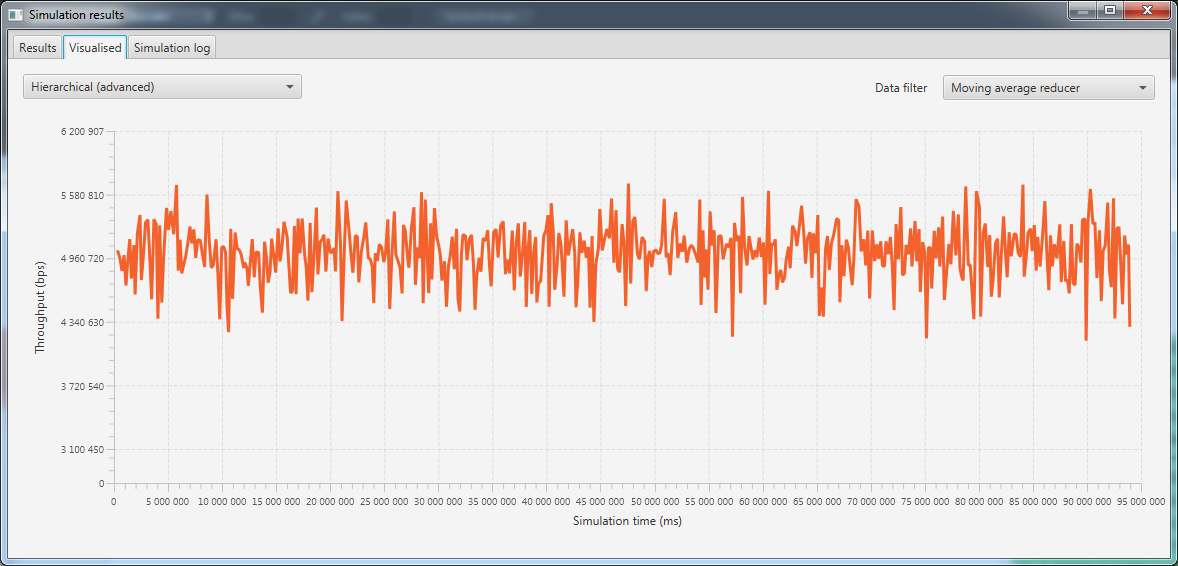
\includegraphics[width=\textwidth]{img/test/mereni_graf_hie.png}
\caption{Graf průběhu rychlosti pro metodu Hierarchical (adv.)}
\label{fig:mereni_graf_hie}
\end{figure}

\begin{figure}[H]
\centering
	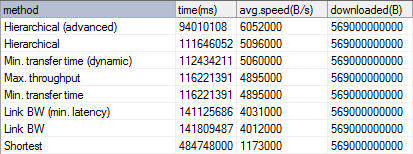
\includegraphics{img/test/tabulka_vysledky.png}
\caption{Zobrazení CSV výsledků}
\label{fig:tabulka_vysledky}
\end{figure}

Na obrázku \ref{fig:mereni_graf_hie} lze vidět ukázku grafu zobrazující rychlost přenosu dat s aplikovaným filtrem \textit{MovingAverageReducer} (viz \ref{filtracevzorku}). Zobrazené exportované výsledky z formátu CSV jsou poté vidět na obrázku \ref{fig:tabulka_vysledky}.

\chapter{Závěr}

Cílem této práce bylo prozkoumat principy fungování distribuovaného souborového systému, navrhnout možnosti využití hierarchického modelu uložení dat a následně implementovat simulátor, který umožní simulaci libovolných modelů distribuovaných souborových systémů. Na závěr měly být pomocí implementovaného simulátoru provedeny měření propustnosti základních modelů distribuovaného souborového systému bez hierarchického modelu uložení dat a s hierarchickým modelem uložení dat.

V praktické části byl navržen a úspěšně implementován simulátor, který umožňuje modelování, měření a porovnávání modelů distribuovaných souborových systémů. Součástí simulátoru je grafické prostředí umožňující modelování systému pomocí drag and drop operací a možnost importovat a exportovat prostředí do souboru. Simulátor podporuje simulaci zatížení linky podle definované charakteristiky propustnosti, která může odpovídat měřením propustnosti provedeným nad reálným systémem. Bylo implementováno celkem 8 modelů simulace, které byly následně otestovány pomocí společného scénáře a naměřené výsledky byly odůvodněny a zhodnoceny v kapitole \ref{testy}. Součástí měření bylo měření vlivu navržené možnosti využití hierarchického modelu uložení dat na propustnost systému, u kterého se na testovaném scénáři výsledná propustnost zvedla téměř o 20\% oproti identické metodě bez použití hierarchického modelu.

Architektura simulátoru spolu s UML diagramy tříd byla popsána v implementační části této práce. Zdrojové kódy jsou detailně okomentovány pomocí javadoc komentářů a doplněny unit testy, které byly průběžně během vývoje používány k ověření správné funkcionality programu. Díky poskytnuté dokumentaci a modulárnímu návrhu lze simulátor v budoucnu rozšířit o další funkcionalitu. Vytvořený simulátor lze provozovat na všech třech hlavních operačních systémech MS Windows, Linux a Mac OS.

Během testování a měření výkonnosti modelů jsem zjistil, že by dále bylo vhodné simulátor rozšířit například o nástroje umožňující automatické generování modelů zapojení distribuovaného souborového systému, generování scénářů simulace z logů reálných systémů nebo přízpůsobit grafické rozhraní pro rozsáhlé systémy s velkým počtem uzlů.

\appendix

\chapter{Použité zkratky}

\begin{itemize}
\item \textbf{SSD} Solid State Drive
\item \textbf{HDD} Hard Disk drive
\item \textbf{JBOD} Just a Buch Of Disks
\item \textbf{RAM} Random Access Memory
\item \textbf{RW} Read Write
\item \textbf{RO} Read Only
\item \textbf{RPC} Remote Procedure Call
\item \textbf{MPI} Message Passing Interface
\item \textbf{LRU} Least Recently Used
\item \textbf{LFU} Least Frequently Used
\item \textbf{FIFO} First In, First Out
\item \textbf{I/O} Input/Output
\item \textbf{XML} eXtensible Markup Language
\item \textbf{UML} Unified Modeling Language
\item \textbf{ADSL} Asymmetric Digital Subscriber Line
\item \textbf{ICMP} Internet Control Message Protocol
\item \textbf{GUI} Graphic User Interface
\item \textbf{VFS} Virtual File System
\item \textbf{CSS} Cascading Style Sheets
\item \textbf{API} Application Programming Interface
\item \textbf{CSV} Comma Separated Values
\end{itemize}

\chapter{Přiložené CD}

Součástí práce je přiložené CD s následujícím obsahem:

\begin{itemize}
\item \textbf{dist} spustitelný JAR soubor
\item \textbf{doc} kopie této práce
	\begin{itemize}
	\item \textbf{javadoc} javadoc dokumentace vygenerovaná ze zdrojových kódů
	\item \textbf{dpsrc} zdrojové kódy práce v \TeX
	\end{itemize}
\item \textbf{Poster} poster k této práci
\item \textbf{prostredi} testované prostředí DFS
\item \textbf{src} zdrojové kódy
	\begin{itemize}
	\item \textbf{main} zdrojové kódy simulátoru
	\item \textbf{test} zdrojové kódy JUnit testů
	\end{itemize}
\end{itemize}

\chapter{Uživatelská příručka}

Tato část slouží jako návod pro uživatele při práci se simulátorem.

\section{Přeložení a spuštění}

Pro běh simulátoru je vyžadováno \textit{JRE} verze alespoň \textit{1.8}\footnote{\url{http://www.oracle.com/technetwork/java/javase/downloads/jre8-downloads-2133155.html}} a přítomnost knihovny \textit{JavaFX} verze \textit{8.0.40} a vyšší na classpath. \textit{JavaFX} je od verze \textit{7u6} součástí \textit{Javy} od \textit{Oracle}.

\subsection{Přeložení}

Pro přeložení simulátoru je nutné mít \textit{JDK} verze alespoň \textit{1.8}\footnote{\url{http://www.oracle.com/technetwork/java/javase/downloads/jdk8-downloads-2133151.html}} a nainstalovaný \textit{Apache Ant}\footnote{\url{https://ant.apache.org/bindownload.cgi}}.

Pro přeložení projektu se musíme nejdřív přepnout do složky se zdrojovými soubory (na přiloženém CD složka \textit{src}). Samotné přeložení poté spustíme příkazem

\begin{verbatim}
ant dist,
\end{verbatim}

\noindent který vytvoří ve složce \textit{dist/lib} JAR soubor \textit{dfs\_simulator.jar}.

\subsection{Spuštění JUnit testů}

JUnit testy ve složce \textit{src/test} lze spustit ze složky \textit{src} příkazem

\begin{verbatim}
ant test,
\end{verbatim}
\noindent který na obrazovce vypíše výstup všech testů.

\subsection{Spuštění}

Pro spuštění projektu slouží dodaný nebo námi vytvořený JAR soubor. Výchozím umístěním JAR souboru je \textit{src/dist/lib/dfs\_simulator.jar} a ze složky \textit{src} ho lze spustit příkazem

\begin{verbatim}
java -jar dist/lib/dfs_simulator.jar.
\end{verbatim}

\section{Vytvoření uzlu}

\begin{figure}
\centering
	\fbox{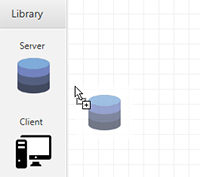
\includegraphics{img/prirucka/vytvoreni_uzel_mys.png}}
\caption{Vytvoření uzlu tažením myší}
\label{fig:p_vytvoreni_uzel_mys}
\end{figure}

\begin{figure}
\centering
	\fbox{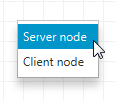
\includegraphics{img/prirucka/vytvoreni_uzel_kontext.png}}
\caption{Vytvoření uzlu přes kontextové menu}
\label{fig:p_vytvoreni_uzel_kontext}
\end{figure}

Vytvoření uzlu typu klient nebo server probíhá tažením myši odpovídajícího prvku z panelu \textit{Library} na modelovací plátno, viz obr. \ref{fig:p_vytvoreni_uzel_mys}. Nově vytvořený uzel je vytvořen na místě, na které byl tažen myší. Alternativně lze vytvořit uzel pomocí pravého tlačítka myši přes kontextové menu, viz obr. \ref{fig:p_vytvoreni_uzel_kontext}.

\subsection{Konfigurace uzlu}

\begin{figure}
\centering
	\fbox{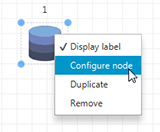
\includegraphics{img/prirucka/konfigurace_uzel.png}}
\caption{Konfigurace uzlu}
\label{fig:p_konfigurace_uzel}
\end{figure}

Vyvolání dialogu pro konfiguraci uzlu lze provést stiskem pravého tlačítka myši nad daným uzlem a vybráním možnosti „Configure node“ (obr. \ref{fig:p_konfigurace_uzel}) nebo dvojklikem myší na uzel.

\subsubsection*{Seznam sousedů}

V konfiguračním dialogu lze v záložce „Node connections“ zobrazit tabulku se seznamem všech sousedů. Spojení se sousedem lze upravit pomocí kontextového menu možností „Alter link“ nebo smazat možností „Delete link“.

\subsection{Popisek uzlu}

Všechny uzly na modelovacím plátně mohou mít zobrazitelný popisek (lze vidět na obr. \ref{fig:p_konfigurace_uzel}), který zároveň představuje unikátní identifikátor uzlu. Skrýt či zobrazit popisek lze přes kontextové menu uzlu vyvolané pravým tlačítkem a vybráním volby „Display label“. Popisek je ve výchozím stavu vždy zobrazen.

\subsection{Přemístění uzlu na plátně}

Všechny uzly, včetně popisků uzlů, lze na plátně libovolně přemístit tažením levým tlačítkem myši. Je-li tažený prvek přemístěn mimo viditelné hranice, je modelovací plátno automaticky rozšířeno. 

\begin{figure}
\centering
	\fbox{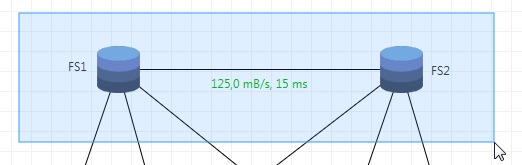
\includegraphics{img/prirucka/hromadny_vyber.png}}
\caption{Hromadný výběr uzlů}
\label{fig:p_hromadny_vyber}
\end{figure}

Pro výběr více prvků najednou lze použít hromadného výběru, který lze vytvořit tažením levého tlačítka myši a obsažením požadovaných prvků ve výběrovém obdélníku, viz obr. \ref{fig:p_hromadny_vyber}. 

Pro přidání dalšího prvku do aktuálního výběru lze použít klávesu \textit{Shift} a provést výběr nad požadovanými prvky. Pro přidání prvku ležícího mimo aktuální výběr nebo odebrání prvku z aktuálního výběru lze použít klávesu \textit{Control} a provést výběr nad daným prvkem či prvky.

\section{Vytvoření spojení}

\begin{figure}
\centering
	\fbox{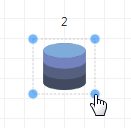
\includegraphics{img/prirucka/vytvoreni_spojeni_rohy.png}}
\caption{Výchozí body pro vytvoření spojení}
\label{fig:p_vytvoreni_spojeni_rohy}
\end{figure}

\begin{figure}
\centering
	\fbox{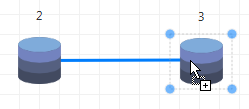
\includegraphics{img/prirucka/vytvoreni_spojeni_ohraniceni.png}}
\caption{Zobrazené ohraničení pro akceptování spojení}
\label{fig:p_vytvoreni_spojeni_ohraniceni}
\end{figure}

Spojení mezi uzly lze vytvořit tažením myší z jednoho ze čtyř modrých kruhů zobrazených při najetí myší nad uzel, viz obr. \ref{fig:p_vytvoreni_spojeni_rohy}. Pro úspěšné spojení musí být spojení přetaženo nad jiný uzel, který kolem sebe zobrazí ohraničení (obr. \ref{fig:p_vytvoreni_spojeni_ohraniceni}), do kterého musí být spojení přetaženo, aby bylo úspěšně vytvořeno.

\subsection{Konfigurace spojení}

\begin{figure}[H]
\centering
	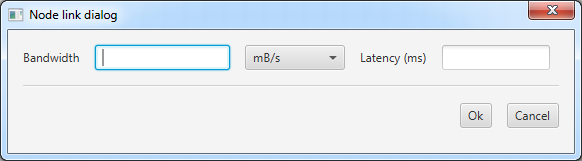
\includegraphics[width=\textwidth]{img/prirucka/vytvoreni_spojeni_dialog.png}
\caption{Dialog konfigurace spojení}
\label{fig:p_vytvoreni_spojeni_dialog}
\end{figure}

Po úspěšném vytvoření spojení mezi uzly je zobrazen dialog (obr. \ref{fig:p_vytvoreni_spojeni_dialog}), pomocí kterého určíme propustnost spoje a jeho latenci. Upravit vlastnosti spojení lze vyvoláním stejného dialogu pomocí volby „Alter link“ z kontextového menu spojení.

\subsection{Zátěžová charakteristika}

\begin{figure}[H]
\centering
	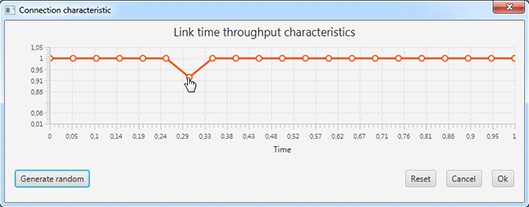
\includegraphics{img/prirucka/spojeni_charakteristika_dialog.png}
\caption{Dialog zátěžové charakteristiky}
\label{fig:p_spojeni_charakteristika_dialog}
\end{figure}

Pro nastavení zátěžové charakteristiky vybraného spojení je třeba vyvolat dialog pomocí volby „Link characteristics“ z kontextového menu spojení. Dialog zátěžové charakteristiky lze vidět na obrázku \ref{fig:p_spojeni_charakteristika_dialog}. 

Charakteristika je definována celkem 21 body a perioda charakteristiky je 60 sekund. Pro upravení propustnosti ve vybraném časovém okamžiku lze bod vertikálně táhnout myší, čímž je upravena hodnota propustnosti spoje. Pomocí tlačítka \textit{Generate random} lze vygenerovat náhodné zatížení.

\subsection{Grafická reprezentace spojení}

\begin{figure}
\centering
	\fbox{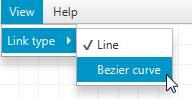
\includegraphics{img/prirucka/menu_typ_spojeni.png}}
\caption{Typ grafického zobrazení spojení}
\label{fig:p_menu_typ_spojeni}
\end{figure}

Spojení mezi uzly lze graficky zobrazit dvěma způsoby a to buď přímkou nebo Bézierovo křivkou. Podobu zobrazeného spojení lze vybrat z hlavního menu aplikace, viz obr. \ref{fig:p_menu_typ_spojeni}.

\section{Úložiště a adresářová struktura}

V konfiguračním dialogu serveru lze spravovat úložiště na daném serveru a jeho adresářovou strukturu.

\subsection{Seznam úložišť}

V záložce „Storage configuration“ lze přidávat nová úložiště a upravovat existující. Tlačítkem „Add storage“ lze přidat nové úložiště. Úložiště jsou zobrazeny v tabulce a vyvoláním kontextového menu pravým tlačítkem lze existující úložiště volbou „Edit storage“ upravit nebo volbou „Delete“ smazat. 

\begin{figure}
\centering
	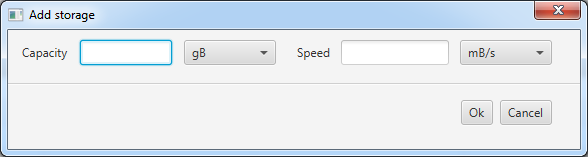
\includegraphics[width=\textwidth]{img/prirucka/uloziste_dialog.png}
\caption{Dialog pro vytvoření nebo úpravu úložiště}
\label{fig:p_uloziste_dialog}
\end{figure}

Vytvoření úložiště nebo úprava existujícího probíhá pomocí dialogu na obr. \ref{fig:p_uloziste_dialog}, který umožňuje nastavení rychlosti úložiště a jeho kapacity.

\subsection{Adresářová struktura}

Záložka „File structure“ v konfiguračním dialogu slouží pro správu adresářové struktury serveru.Výchozí složkou je kořenová složka \textit{/}, kterou nelze smazat ani upravovat. Přidání souboru či složky do kořenové složky probíhá přes kontextové menu volbou „New file“ a „New subdirectory“ pro přidání souboru, respektive složky. Upravit existující soubor či složku lze pomocí možnosti „Edit“, která vyvolá odpovídající dialog.

\subsubsection*{Umístění objektu na úložiště}

Libovolný objekt může být umístěn na libovolném úložišti. Výběr úložiště pro objekt lze provést nabídkou „Select mount device“ z kontextového menu objektu, která vyvolá dialog pro výběr úložiště. Pokud potomci nemají explicitně stanovené úložiště, na kterém jsou umístěni, potom mohou úložiště zdědit od prvního předka, který má vybrané úložiště.

\subsubsection*{Replikace souborů}

\begin{figure}[H]
\centering
	\fbox{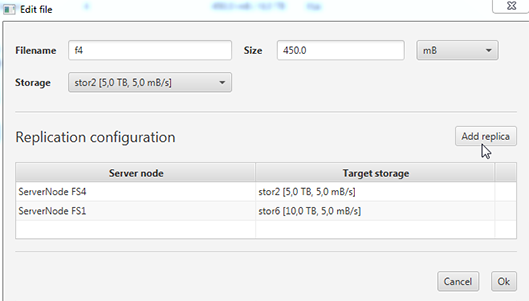
\includegraphics{img/prirucka/uloziste_soubor_replikace.png}}
\caption{Dialog pro vytváření a úpravu souborů}
\label{fig:p_uloziste_soubor_replikace}
\end{figure}

V dialogu pro vytváření souborů (obr. \ref{fig:p_uloziste_soubor_replikace} lze zároveň definovat, jak bude soubor replikován. Přidání nové repliky probíhá tlačítkem „\textbf{Add replica}“, které vyvolá dialog pro výběr cílového serveru a cílového úložiště, na které má být soubor replikován. V seznamu replik lze repliku odstranit pomocí kontextového menu a volby „Delete replica“.

\section{Plánování a spuštění simulace}

\begin{figure}[H]
\centering
	\fbox{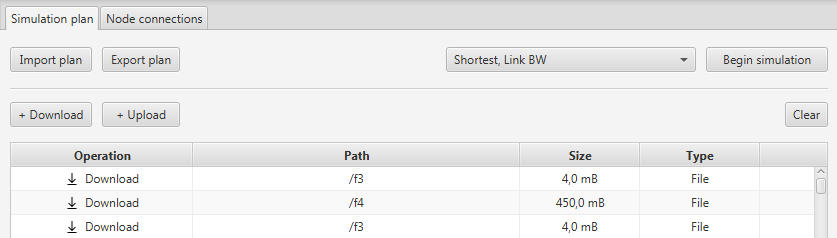
\includegraphics[width=\textwidth]{img/prirucka/klient_plan_simulace.png}}
\caption{Simulační plán}
\label{fig:p_klient_plan_simulace}
\end{figure}

Plánování a spuštění simulace probíhá v záložce „Simulation plan“ (obr. \ref{fig:p_klient_plan_simulace} z konfiguračního dialogu konkrétního klienta. Tlačítkem „\textbf{+ Download}“ je vyvolán dialog, pomocí kterého můžeme vybrat 1 či více souborů, které mají být staženy. Tlačítkem „\textbf{+ Upload}“ je vyvolán dialog, ve kterém můžeme definovat název souboru, velikost a umístění, do kterého má být nahrán.

\subsection{Výběr typu simulace}

\begin{figure}[H]
\centering
	\fbox{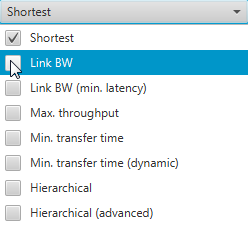
\includegraphics{img/prirucka/klient_plan_typy_simulace.png}}
\caption{Výběr typu simulace}
\label{fig:p_klient_plan_typy_simulace}
\end{figure}

Pomocí seznamu na obr. \ref{fig:p_klient_plan_typy_simulace} lze vybrat 1 či více typů simulace, které mají být provedeny nad vytvořeným plánem. 

\subsection{Spuštění simulace}

Tlačítkem „\textbf{Begin simulation}“ spustíme simulaci vybraných typů podle společného plánu. Po spuštění simulace je zobrazen dialog, který informuje uživatele o průběhu simulace.

\subsection{Vizualizace simulace}

\begin{figure}
\centering
	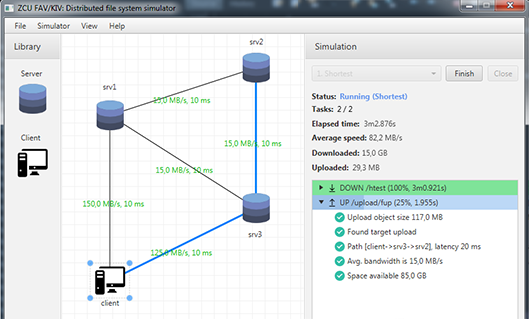
\includegraphics{img/prirucka/prubeh_vizualizace_simulace.png}
\caption{Vizualizace simulace}
\label{fig:p_prubeh_vizualizace_simulace}
\end{figure}

Vizualizace průběhu simulace je viditelná na obr. \ref{fig:p_prubeh_vizualizace_simulace}. V postranním panelu na pravé straně lze vidět několik položek:

\begin{itemize}
\item \textbf{Status} - aktuální status průběhu simulace,
\item \textbf{Tasks} - počet zpracovaných / počet celkových položek simulačního plánu,
\item \textbf{Elapsed time} - čas, který byl potřebný k přenesení zpracovaných položek,
\item \textbf{Average speed} - průměrná rychlost přenosu zpracovaných položek,
\item \textbf{Downloaded} - množství stažených dat zpracovanými položkami,
\item \textbf{Uploaded} - množství nahraných dat zpracovanými položkami.
\end{itemize}

\noindent U každé aktuálně zpracovávané položky je zároveň zvýrazněna cesta (na obr. \ref{fig:p_prubeh_vizualizace_simulace} modrou barvou), přes kterou jsou přenášena data.

Pokud si nepřejeme čekat na výsledky do doběhnutí vizualizace, lze použít tlačítko „\textbf{Finish}“, které urychlí vizualizaci a zobrazí výsledky.

\section{Výsledky simulace}

Po dokončení vizualizace simulace je uživateli zobrazeno dialogové okno s výsledky simulace. 

\subsection{Export do CSV}

\begin{figure}
\centering
	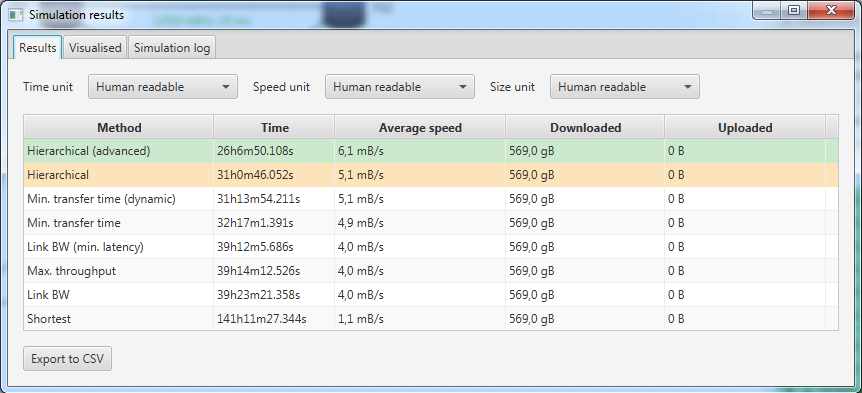
\includegraphics[width=\textwidth]{img/prirucka/simulace_vysledky.png}
\caption{Výsledky simulace}
\label{fig:p_simulace_vysledky}
\end{figure}

Naměřené výsledky lze prohlížet v tabulce v záložce „Results“ (obr. \ref{fig:p_simulace_vysledky}). Tabulka má celkem 5 sloupců a to:

\begin{itemize}
\item \textbf{Method} - název testované metody,
\item \textbf{Time} - celkový čas přenosu dat,
\item \textbf{Average speed} - průměrná rychlost,
\item \textbf{Downloaded} - objem stažených dat,
\item \textbf{Uploaded} - objem nahraných dat.
\end{itemize}

\noindent Řádky tabulky jsou seřazeny od nejlepšího času po nejhorší a dva nejlepší výsledky jsou zvýrazněny zelenou respektive oranžovou barvou.

Násobky naměřených hodnot lze vybrat pomocí odpovídajících select boxů - „Time unit“ pro násobky času, „Speed unit“ pro násobky rychlosti a „Size unit“ pro násobky velikosti. Výchozí hodnotou všech 3 je „Human readable“, která převádí hodnoty na snadno čitelný formát, ovšem ne vždy úplně přesný (zaokrouhlování rychlosti a velikosti).

Tlačítkem „\textbf{Export to CSV}“ lze tabulku exportovat do vybraného souboru. Hodnoty budou exportovány ve stejném formátu, v jakém jsou aktuálně zobrazeny v tabulce (tzn. s vybranými násobky). 

\subsection{Graf průběhu rychlosti}

\begin{figure}
\centering
	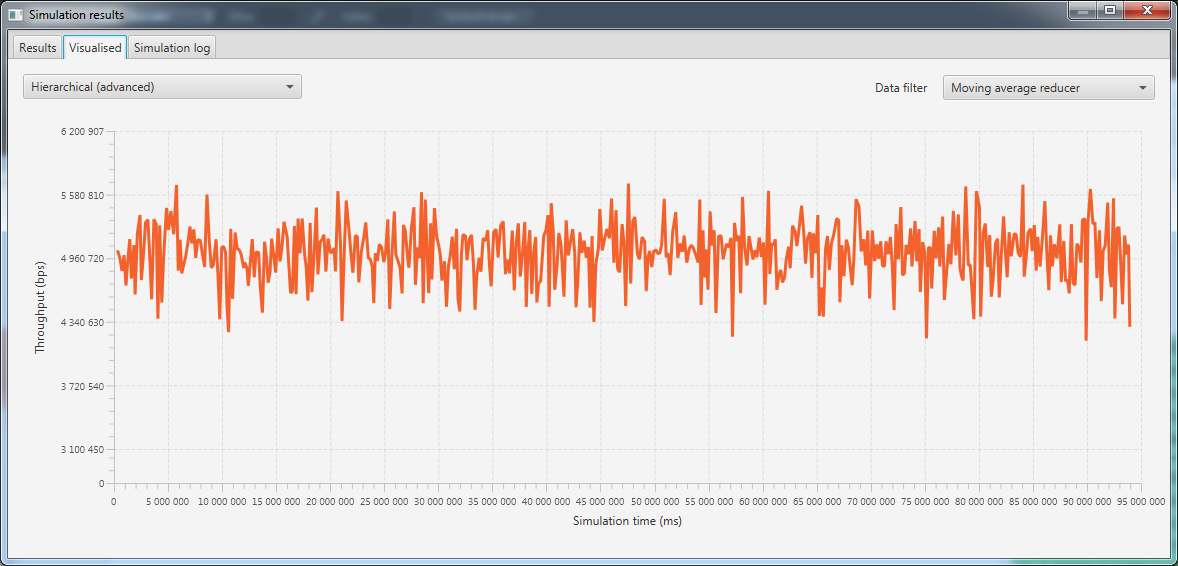
\includegraphics[width=\textwidth]{img/prirucka/simulace_graf.png}
\caption{Graf průběhu rychlosti}
\label{fig:p_simulace_graf}
\end{figure}

V záložce „Visualised“ lze vidět spojnicový graf (obr. \ref{fig:p_simulace_graf}), zobrazující průběh rychlosti přenosu v závislosti na uběhnutém času. Na ose X je čas v milisekundách a na ose Y je rychlost přenosu v B/s. 

\subsubsection*{Filtr vzorků}

Naměřené vzorky rychlosti jsou ve výchozím stavu dodatečně filtrovány, aby jejich vykreslení nebylo příliš náročné. Filtr lze zvolit select boxem s popiskem „Data filter“ a jsou na výběr následující filtry:

\begin{itemize}
\item \textbf{No filter (CPU Intensive)} vrací všechny vzorky, náročný, přesný ale ne příliš vhodný pokud máme hodně vzorků,
\item \textbf{Douglas-Peucker} využívá Douglas-Peucker algoritmu \cite{douglaspeuckeralg},
\item \textbf{Radial distance} funguje na bázi eukleidovské vzdálenosti bodů,
\item \textbf{Moving average} výchozí filtr - dělí hodnoty do časových intervalů a pro každý časový interval počítá průměr hodnot. Filtrace probíhá rychle i pro větší množství vzorků.
\end{itemize}

\subsection{Detaily simulace}

V záložce „Simulation log“ je k zobrazení log průběhu simulace, který zaznamenává některé důležité události při provádění jednotlivých požadavků. Každý záznam má na začátku v hranaté závorce časové razítko.

\section{Import a export prostředí}

Modelovaný systém a simulační plán lze exportovat do XML souboru, z kterého lze později načíst.

\subsection{Modelované prostředí}

\begin{figure}
\centering
	\fbox{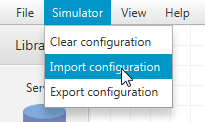
\includegraphics{img/prirucka/simulator_import_export.png}}
\caption{Import a export prostředí}
\label{fig:p_simulator_import_export}
\end{figure}

Modelované prostředí lze exportovat pomocí nabídky v hlavním menu (obr. \ref{fig:p_simulator_import_export}) \textit{Simulator - Export configuration}. Následně je zobrazen dialog, pomocí kterého je vybrán cílový soubor. Import probíhá obdobným způsobem nabídkou \textit{Simulator - Import configuration}, která vyzve uživatele k vybrání souboru s exportovaným stavem.

\subsection{Simulační plán}

Ve stejném dialogu, ve kterém se vytváří simulační plán (obr. \ref{fig:p_klient_plan_simulace}) je zároveň možnost plán uložit do externího souboru nebo ho z něj načíst. Tlačítkem „\textbf{Import plan}“ lze provést importování simulačního plánu z externího souboru a tlačítkem „\textbf{Export plan}“ lze uložit stávající plán do souboru.

\listoffigures

\listoftables


% 
% PRO ANGLICKOU SAZBU JE NUTNÉ ZMĚNIT
% CITAČNÍ STYL!
%
\bibliographystyle{csplainnatkiv}
{\raggedright\small
\bibliography{literatura}
}

\end{document}
